%% Wiley New Journal Design (NJD) v5 -- settings for Biometrical Journal: STIX font,
%% single column, numbered (AMA) reference style as supplied with the template.
%% Compile with XeLaTeX (fontspec loads the bundled STIX fonts from ./Fonts):
%%   latexmk -xelatex main        or        xelatex main; bibtex main; xelatex main; xelatex main
%% On Overleaf: Menu -> Compiler -> XeLaTeX. This cannot be set from within the file.
%% Tables in tables/ are generated from results/*.csv by R/make_tables.R.
\RequirePackage{iftex}
\ifXeTeX\else
  \errmessage{This class needs XeLaTeX. On Overleaf set Menu > Compiler > XeLaTeX}
\fi
%% TeX Live >= 2025: etex.sty no longer defines \reserveinserts once the kernel's
%% extended allocation is in use, but WileyNJDv5.cls (line 356) calls it. Load etex
%% first as its warning suggests, and fall back to a no-op if it still bails out;
%% the modern kernel allocates inserts from the extended pool without reservation.
\RequirePackage{etex}
\providecommand{\reserveinserts}[1]{}
\documentclass[STIX1COL]{WileyNJDv5}
%% Author--year references in APA style (Biometrical Journal). The class's APA
%% option needs Wiley's NJDapacite.sty and WileyNJD-APA.bst, which are not
%% distributed with this template, so the standard apacite package is used with
%% natbib citation commands (\citet, \citep, \citealt).
\usepackage[natbibapa]{apacite}
\bibliographystyle{apacite}
\makeatletter
\NAT@longnamesfalse % ``et al.'' from the first citation of a work with three or more authors
\renewcommand\refname{REFERENCES}
\renewcommand{\bibfont}{\reset@font\fontfamily{\rmdefault}\fontsize{8.5}{11}\selectfont\baselineskip=10\p@}
\makeatother

\usepackage{bm}
\usepackage{booktabs}
\usepackage{enumitem}
\usepackage{tikz}
\usetikzlibrary{positioning,arrows.meta,shapes.geometric,fit,calc}
\graphicspath{{figures/}}

%% ---- notation macros
\newcommand{\Dir}{\mathrm{Dir}}
\newcommand{\Beta}{\mathrm{Beta}}
\newcommand{\Mult}{\mathrm{Multinomial}}
\newcommand{\E}{\mathbb{E}}
\renewcommand{\Pr}{\mathrm{Pr}}
\newcommand{\Var}{\mathrm{Var}}
\newcommand{\Cov}{\mathrm{Cov}}
\newcommand{\thmtone}{\ref{thm:t1e}} % wrapper so the uppercased appendix heading keeps the label intact
\newcommand{\ind}{\mathbf{1}}
\newcommand{\bpi}{\bm{\pi}}
\newcommand{\balpha}{\bm{\alpha}}
\newcommand{\bw}{\mathbf{w}}
\newcommand{\bx}{\mathbf{x}}
\newcommand{\bc}{\mathbf{c}}
\newcommand{\by}{\mathbf{y}}
\newcommand{\bY}{\mathbf{Y}}
\newcommand{\bmm}{\mathbf{m}}
\newcommand{\cR}{\mathcal{R}}
\newcommand{\cJ}{\mathcal{J}}
\newcommand{\cA}{\mathcal{A}}
\newcommand{\cW}{\mathcal{W}}
\newcommand{\cC}{\mathcal{C}}
\newcommand{\PCS}{\mathrm{PCS}}
\newcommand{\PPoS}{\mathrm{PPoS}}

%% ---- production fields (filled in by the journal)
\articletype{Research Article}
\received{Added at production}
\revised{Added at production}
\accepted{Added at production}
\journal{Biometrical Journal}
\volume{00}
\copyyear{2026}
\startpage{1}
\raggedbottom

\begin{document}

\title{A Bayesian seamless phase II/III dose-selection design with a weighted composite selection endpoint and co-primary confirmatory endpoints}

\author[1,2]{Zerong Chen}

\authormark{CHEN}
\titlemark{Seamless design with composite selection and co-primary confirmation}

\address[1]{\orgdiv{National Heart and Lung Institute}, \orgname{Imperial College London}, \orgaddress{\state{London}, \country{United Kingdom}}}
\address[2]{\orgdiv{Imperial Clinical Trials Unit}, \orgname{Imperial College London}, \orgaddress{\state{London}, \country{United Kingdom}}}

\corres{Zerong Chen, National Heart and Lung Institute, Imperial College London, London, United Kingdom. \email{z.chen@imperial.ac.uk}}

\abstract[Abstract]{Confirmatory trials with $K$ binary co-primary endpoints require every endpoint to succeed, so the type II error inflates with $K$ and the sample size rises accordingly. In a seamless phase II/III dose-selection design this cost is paid once per candidate dose at the selection stage. We propose a design in which the $M$ doses are compared at the interim on a single pre-specified weighted composite of the binary components, and the selected dose is confirmed on the full co-primary criterion with the stage-1 data included. Both functionals are projections of the same Dirichlet--multinomial cell-probability vector, so the inter-endpoint dependence is determined by the model rather than assumed. We prove that the probability of a false co-primary claim is at most $\alpha$ for every configuration of effects and for any selection rule, futility rule and stage-2 sample size, by a closed test over all dose--endpoint hypotheses with stage-wise $p$-values combined by the inverse-normal rule, computed exactly through a closed-form shortcut; closing each endpoint separately over doses does not control this error, and we quantify the inflation. Under parallel dose effects a second-moment argument brackets the ratio of stage-1 sample sizes needed for a given selection accuracy below one, and we characterise the configurations in which the composite gate fails: discordance between the composite and co-primary optima, and failure on a single component, which a composite registers weakly. In simulation calibrated to a four-serogroup meningococcal vaccine example, the design reaches a claim probability of 0.80--0.90 with about 10\% fewer expected subjects than a co-primary-gated seamless design under parallel dose effects (9--12\% with uniform weights, 5--9\% with the weights the design rule selects), saves little or nothing when the dose-discriminating information is concentrated on one endpoint, and is inferior when the optimum is a trade-off between endpoints. A design rule based on the frontier of claim probability against expected sample size is given.}

\keywords{adaptive seamless design; closed testing; co-primary endpoints; composite endpoint; Dirichlet--multinomial; dose selection; treatment selection}

\jnlcitation{\cname{\author{Z. Chen}}. \ctitle{A Bayesian seamless phase II/III dose-selection design with a weighted composite selection endpoint and co-primary confirmatory endpoints.} \cjournal{\it Biometrical Journal} \cvol{2026;00(00):1--29}.}

\maketitle

\section{Introduction}\label{sec:intro}

Some treatments are required to work on several targets at once, and the confirmatory trial then has several primary endpoints that must all show an effect. Multivalent vaccines are the clearest case: a quadrivalent meningococcal conjugate vaccine is licensed on serogroup-specific immunogenicity, and success means non-inferiority to the licensed comparator on each of serogroups A, C, W and Y\cite{yang2024,ostergaard2009}. Endpoints of this kind are called co-primary. They are tested by the intersection--union principle, each at the nominal level $\alpha$, with success declared only if every test rejects\cite{berger1982}; no multiplicity adjustment is required, but the type II error accumulates, the power of the conjunction being at most the smallest marginal power and well below it when the endpoints are weakly correlated, and the sample size rises with the number of endpoints\cite{offen2007,chuangstein2007,sozu2010,hamasaki2018}.

When the confirmatory trial is preceded by the selection of one of several candidate doses or formulations, an adaptive seamless phase II/III design can combine the two steps\cite{bauer1994,stallard2003,posch2005,bretz2006,jennison2007,stallard2011}. Stage 1 randomises to all candidates and control, an interim analysis selects one candidate, stage 2 continues with the selected candidate and control, and the final analysis uses the data of both stages. Type I error control despite the data-dependent selection is obtained by a combination test over stages together with a closed test over candidates\cite{marcus1976,bauer1994,hommel2001,posch2005,bretz2006}. Dose optimisation has made this setting topical\cite{fda2024,li2024,liu2026}, and Yang et al\cite{yang2024} have proposed a Bayesian seamless design for co-primary endpoints in which the selection stage applies the co-primary criterion to every candidate and the stage-2 sample size is chosen by predictive power.

With co-primary endpoints the price of the conjunction is paid at the selection stage as well as at the final analysis, and it is paid once for each candidate. Ranking candidates on the co-primary criterion means ranking them on their weakest endpoint, and with the small stage-1 sample sizes typical of a selection stage the weakest endpoint is a noisy statistic that discards the information in the other endpoints. The question of this paper is whether the selection stage can use a different functional of the same endpoints, one that pools the information across them, without compromising the confirmatory claim.

Selecting on an endpoint other than the confirmatory one is established practice in seamless designs: short-term or surrogate endpoints have been used to select treatments that are then confirmed on a long-term endpoint\cite{stallard2010,friede2011,kunz2014}, and progression-free survival has been used to select a subpopulation confirmed on overall survival\cite{jenkins2011}. There the selection endpoint is available earlier, and the error-control argument is that the final test is valid whatever the selection rule. The switch proposed here is of a different kind. Both functionals are computed from the same $K$ binary responses measured on the same subjects: selection uses a pre-specified weighted composite of the components, the weighted responder score of Zaslavsky\cite{zaslavsky2013}, and confirmation uses the conjunctive co-primary criterion. Because the composite and the component success probabilities are all linear functionals of the multinomial vector of cell probabilities over the $2^K$ response patterns, a single Dirichlet--multinomial model\cite{thall1995,yang2024} delivers the posterior of every quantity used in either stage, and the dependence between endpoints is a property of the shared cells rather than an assumption. Selection is Bayesian; confirmation is a frequentist test with the stage-1 data included.

The contribution is as follows. Section~\ref{sec:design} sets out the design and proves (Theorem~\ref{thm:t1e}) that the probability of a false co-primary claim is at most $\alpha$ for every configuration of true effects and for any selection rule, futility rule and stage-2 sample size. The proof uses a closed test over doses in which each intersection hypothesis is tested by an intersection--union test, and we show that the more obvious alternative, closing each endpoint separately, does not control the error when different doses fail on different endpoints. Section~\ref{sec:saving} gives the conditions under which the composite reaches a target probability of correct selection with a smaller stage-1 sample than the co-primary criterion, a concordance requirement on the weights and a second-moment bracket for the ratio of stage-1 sizes under parallel dose effects, and identifies the configurations in which the composite is worse. Section~\ref{sec:sim} reports a simulation study calibrated to the meningococcal example, comparing the proposed design with a seamless design that applies the co-primary criterion at both stages, from selection accuracy through the futility rule to the final claim, and Section~\ref{sec:rule} turns the findings into a design rule based on the frontier of claim probability against expected sample size. Section~\ref{sec:disc} discusses limitations and extensions. Proofs are in the Appendix, and R code reproducing every table and figure is provided.

\section{Motivating example}\label{sec:motivation}

Quadrivalent meningococcal conjugate vaccines are licensed on immunogenicity, and the confirmatory standard is a set of serogroup-specific binary endpoints that must all be met. Yang et al\cite{yang2024} describe a trial of a quadrivalent meningococcal tetanus toxoid-conjugate vaccine in which seroresponse for each of serogroups A, C, W and Y was a co-primary endpoint, success requiring non-inferiority to the licensed comparator on all four with a margin of $-10$ percentage points, and report comparator seroresponse rates of $0.425$, $0.497$, $0.448$ and $0.434$. Four binary endpoints in conjunction is exactly the setting in which the type II error of a co-primary analysis inflates and the sample size rises accordingly.

Upstream of such a trial sits a formulation-selection stage. {\O}stergaard et al\cite{ostergaard2009} compared five candidate MenACWY-TT formulations, differing in polysaccharide content and conjugation method, against a licensed ACWY polysaccharide vaccine in two open-label studies of 50 adults aged 18--25 and 125 adolescents aged 15--19, with the percentage of serum bactericidal antibody responders to each of serogroups A, C, W-135 and Y as the immunogenicity endpoints. Responder percentages did not differ from control for any formulation on any serogroup, with one exception: serogroup A was lower after one formulation. The selection problem is therefore $M=5$ candidates and $K=4$ binary components, $2^K=16$ response patterns per subject, and a concurrent control; and its outcome was, in effect, a judgement over four responder rates per formulation made on 25--35 subjects per arm.

Three features of this setting make it the natural home for the design proposed here. First, the components are positively dependent, since they are responses of the same immune system to conjugates of the same carrier, and a better formulation tends to be better on every serogroup; a scalar summary of the four responder rates therefore carries most of the information that distinguishes formulations, and a selection rule that applies the conjunctive criterion to each candidate discards it. Second, the components have a clinically meaningful weighting: serogroup-specific disease burden differs by age and region, so a weighted responder composite of the kind introduced by Zaslavsky\cite{zaslavsky2013} is interpretable and can be fixed from epidemiological data before the trial. Third, the development ran as a small open-label formulation study followed by separate confirmatory trials; a seamless design that randomises the candidates and control in stage 1, selects on the composite, continues the selected formulation and control into stage 2, and confirms on the four co-primary non-inferiority endpoints with the stage-1 data included, is the obvious alternative, and the question the paper answers is what it costs in error control and what it saves in sample size.

The same example supplies the design's principal caveat. The single-serogroup shortfall seen for one formulation is a failure on one component with adequate responses on the other three, and a composite that averages the four responder rates registers it weakly. Section~\ref{sec:e2e} quantifies this: the composite gate proceeds to stage 2 far more often than a conjunctive gate when one component is inert, and the error rate is protected only by the final co-primary test. Whether that cost is acceptable depends on how plausible single-serogroup failure is for the candidates at hand, and the design rule of Section~\ref{sec:rule} places it in the scenario set for that reason.

The simulation study of Section~\ref{sec:sim} uses the comparator seroresponse rates above so that its sample sizes are on the scale of this application, but it tests superiority ($\delta_k=0$) rather than non-inferiority with $\delta_k=-0.10$; the framework accommodates either, and a re-analysis of the formulation study under the non-inferiority margin is the intended illustration.

\section{The design}\label{sec:design}

\subsection{Setting and notation}

Consider a randomised two-stage seamless phase II/III trial comparing $M$ doses, or formulations, $a=1,\dots,M$ of an experimental agent with a concurrent control $C$ on $K$ binary component endpoints; we say ``doses'' throughout, but no ordering of the arms is used. Stage 1 randomises $n_1$ subjects to each of the $M+1$ arms. At the interim analysis at most one dose $a^\star$ is selected. Stage 2 randomises $n_2$ subjects to each of $a^\star$ and $C$. The final analysis pools both stages for $a^\star$ and $C$. Figure~\ref{fig:schematic}(a) shows the flow of the trial, and Figure~\ref{fig:schematic}(b) the relation between the two functionals on which the two stages act.

\begin{figure}
\centering
\resizebox{\textwidth}{!}{%% Schematic of the design (Figure 1). Input from body.tex; requires tikz with
%% libraries positioning, arrows.meta, shapes.geometric, fit, calc (loaded in main.tex).
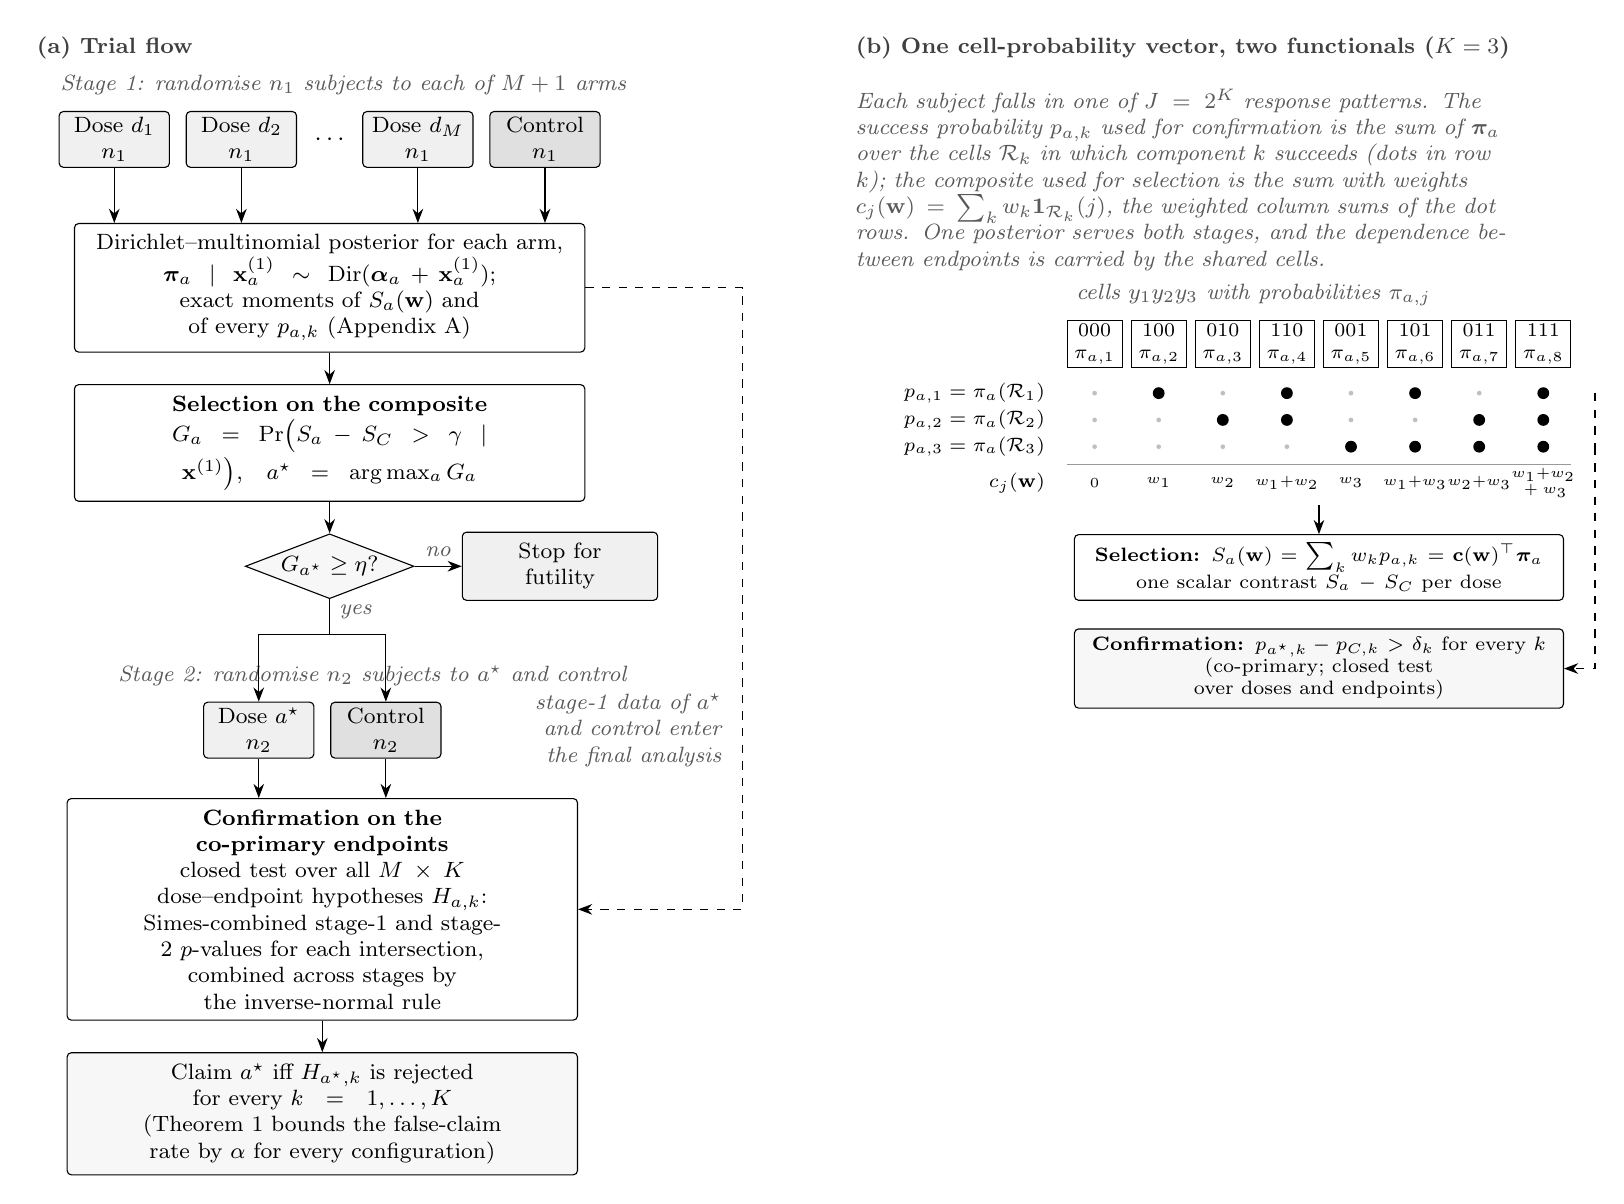
\begin{tikzpicture}[
  font=\footnotesize,
  >={Stealth[length=1.8mm]},
  arm/.style={draw, rounded corners=1.5pt, minimum width=14mm, minimum height=6.5mm,
              align=center, fill=black!6, inner sep=2pt},
  blk/.style={draw, rounded corners=1.5pt, align=center, inner sep=4pt, text width=62mm, fill=white},
  gate/.style={draw, diamond, aspect=2.6, align=center, inner sep=1pt, fill=black!3},
  lab/.style={font=\footnotesize\itshape, text=black!65},
  ptitle/.style={font=\footnotesize\bfseries, text=black!75},
  pat/.style={draw, minimum width=11mm, minimum height=6mm, inner sep=1pt, font=\scriptsize, align=center},
  fun/.style={draw, rounded corners=1.5pt, align=center, inner sep=3pt, font=\scriptsize, text width=34mm},
]
%% ---------------------------------------------------------------- panel (a)
\node[ptitle, anchor=west] (pa) at (0,0) {(a) Trial flow};
% stage 1 arms
\node[arm, below=8mm of pa.west, anchor=north west, xshift=4mm] (d1) {Dose $d_1$\\ $n_1$};
\node[arm, right=2mm of d1] (d2) {Dose $d_2$\\ $n_1$};
\node[right=1mm of d2, font=\small] (dots) {$\cdots$};
\node[arm, right=1mm of dots] (dM) {Dose $d_M$\\ $n_1$};
\node[arm, right=2mm of dM, fill=black!12] (c1) {Control\\ $n_1$};
\node[lab, above=0.8mm of d1.north west, anchor=south west, xshift=-1mm] {Stage 1: randomise $n_1$ subjects to each of $M+1$ arms};
% posterior
\node[blk, below=7mm of $(d1.south)!0.5!(c1.south)$] (post)
  {Dirichlet--multinomial posterior for each arm,\\
   $\bpi_a\mid\bx_a^{(1)}\sim\Dir(\balpha_a+\bx_a^{(1)})$;\\
   exact moments of $S_a(\bw)$ and of every $p_{a,k}$ (Appendix~A)};
% composite gate
\node[blk, below=4mm of post] (comp)
  {\textbf{Selection on the composite}\\
   $G_a=\Pr\big(S_a-S_C>\gamma\mid\bx^{(1)}\big)$,\quad $a^\star=\arg\max_a G_a$};
\node[gate, below=4mm of comp] (dec) {$G_{a^\star}\ge\eta$?};
\node[blk, text width=22mm, right=6mm of dec, fill=black!6] (stop) {Stop for\\ futility};
% stage 2 arms
\node[arm, below=13mm of dec, xshift=-9mm] (a2) {Dose $a^\star$\\ $n_2$};
\node[arm, right=2mm of a2, fill=black!12] (c2) {Control\\ $n_2$};
\node[lab, above=0.8mm of a2.north west, anchor=south west, xshift=-12mm] {Stage 2: randomise $n_2$ subjects to $a^\star$ and control};
% final analysis
\node[blk, below=5mm of $(a2.south)!0.5!(c2.south)$] (fin)
  {\textbf{Confirmation on the co-primary endpoints}\\
   closed test over all $M\times K$ dose--endpoint hypotheses $H_{a,k}$:\\
   Simes-combined stage-1 and stage-2 $p$-values for each intersection,\\
   combined across stages by the inverse-normal rule};
\node[blk, below=4mm of fin, fill=black!3] (claim)
  {Claim $a^\star$ iff $H_{a^\star,k}$ is rejected for every $k=1,\dots,K$\\
   (Theorem~1 bounds the false-claim rate by $\alpha$ for every configuration)};
% arrows
\foreach \n in {d1,d2,dM,c1} \draw[->] (\n.south) -- ($(\n.south |- post.north)$);
\draw[->] (post) -- (comp);
\draw[->] (comp) -- (dec);
\draw[->] (dec) -- node[above, lab] {no} (stop);
\draw[->] (dec) -- node[right, lab, pos=0.35] {yes} ($(dec.south)+(0,-4.5mm)$) -| (a2.north);
\draw[->] ($(dec.south)+(0,-4.5mm)$) -| (c2.north);
\foreach \n in {a2,c2} \draw[->] (\n.south) -- ($(\n.south |- fin.north)$);
\draw[->] (fin) -- (claim);
% stage-1 data re-used
\coordinate (ru) at ($(post.east)+(20mm,0)$);
\draw[->, dashed] (post.east) -- (ru) -- (ru |- fin.east) -- (fin.east);
\node[lab, align=right, anchor=east] at ($(ru |- a2.east)+(-1.5mm,0)$) {stage-1 data of $a^\star$\\ and control enter\\ the final analysis};
%% ---------------------------------------------------------------- panel (b)
\begin{scope}[xshift=104mm]
\node[ptitle, anchor=west] (pb) at (0,0) {(b) One cell-probability vector, two functionals ($K=3$)};
\node[lab, below=4mm of pb.west, anchor=north west, text width=86mm] (btxt)
  {Each subject falls in one of $J=2^K$ response patterns. The success probability $p_{a,k}$ used for confirmation is the
   sum of $\bpi_a$ over the cells $\cR_k$ in which component $k$ succeeds (dots in row $k$); the composite used for selection
   is the sum with weights $c_j(\bw)=\sum_k w_k\ind_{\cR_k}(j)$, the weighted column sums of the dot rows. One posterior serves both stages, and the dependence between
   endpoints is carried by the shared cells.};
% the J = 8 cells, ordered as j = 1 + y_1 + 2 y_2 + 4 y_3
\node[pat, minimum width=7mm, below=5mm of btxt.south west, anchor=north west, xshift=28mm] (c1) {$000$\\ $\pi_{a,1}$};
\node[pat, minimum width=7mm, right=1mm of c1] (c2) {$100$\\ $\pi_{a,2}$};
\node[pat, minimum width=7mm, right=1mm of c2] (c3) {$010$\\ $\pi_{a,3}$};
\node[pat, minimum width=7mm, right=1mm of c3] (c4) {$110$\\ $\pi_{a,4}$};
\node[pat, minimum width=7mm, right=1mm of c4] (c5) {$001$\\ $\pi_{a,5}$};
\node[pat, minimum width=7mm, right=1mm of c5] (c6) {$101$\\ $\pi_{a,6}$};
\node[pat, minimum width=7mm, right=1mm of c6] (c7) {$011$\\ $\pi_{a,7}$};
\node[pat, minimum width=7mm, right=1mm of c7] (c8) {$111$\\ $\pi_{a,8}$};
\node[lab, above=0.5mm of c1.north west, anchor=south west] {cells $y_1y_2y_3$ with probabilities $\pi_{a,j}$};
% membership rows: a dot where component k succeeds in cell j
\coordinate (r1) at ($(c1.south)+(0,-3.2mm)$);
\coordinate (r2) at ($(c1.south)+(0,-6.6mm)$);
\coordinate (r3) at ($(c1.south)+(0,-10.0mm)$);
\coordinate (rc) at ($(c1.south)+(0,-14.6mm)$);
\foreach \j/\m in {1/0,2/1,3/0,4/1,5/0,6/1,7/0,8/1}
  {\ifnum\m=1 \fill (c\j |- r1) circle (0.75mm); \else \fill[black!25] (c\j |- r1) circle (0.3mm); \fi}
\foreach \j/\m in {1/0,2/0,3/1,4/1,5/0,6/0,7/1,8/1}
  {\ifnum\m=1 \fill (c\j |- r2) circle (0.75mm); \else \fill[black!25] (c\j |- r2) circle (0.3mm); \fi}
\foreach \j/\m in {1/0,2/0,3/0,4/0,5/1,6/1,7/1,8/1}
  {\ifnum\m=1 \fill (c\j |- r3) circle (0.75mm); \else \fill[black!25] (c\j |- r3) circle (0.3mm); \fi}
\node[font=\scriptsize, anchor=east] at ($(c1.west |- r1)+(-1.5mm,0)$) {$p_{a,1}=\pi_a(\cR_1)$};
\node[font=\scriptsize, anchor=east] at ($(c1.west |- r2)+(-1.5mm,0)$) {$p_{a,2}=\pi_a(\cR_2)$};
\node[font=\scriptsize, anchor=east] at ($(c1.west |- r3)+(-1.5mm,0)$) {$p_{a,3}=\pi_a(\cR_3)$};
% composite weights c_j(w): the weighted column sums of the dot rows
\node[font=\scriptsize, anchor=east] at ($(c1.west |- rc)+(-1.5mm,0)$) {$c_j(\bw)$};
\node[font=\tiny, align=center] at (c1 |- rc) {$0$};
\node[font=\tiny, align=center] at (c2 |- rc) {$w_1$};
\node[font=\tiny, align=center] at (c3 |- rc) {$w_2$};
\node[font=\tiny, align=center] at (c4 |- rc) {$w_1{+}w_2$};
\node[font=\tiny, align=center] at (c5 |- rc) {$w_3$};
\node[font=\tiny, align=center] at (c6 |- rc) {$w_1{+}w_3$};
\node[font=\tiny, align=center] at (c7 |- rc) {$w_2{+}w_3$};
\node[font=\tiny, align=center] at (c8 |- rc) {$w_1{+}w_2$\\ ${}+w_3$};
\draw[black!40] ($(c1.west |- rc)+(0,2.3mm)$) -- ($(c8.east |- rc)+(0,2.3mm)$);
% selection and confirmation
\coordinate (mid) at ($(c4.east)!0.5!(c5.west)$);
\coordinate (sN) at ($(mid |- rc)+(0,-6.5mm)$);
\node[fun, text width=60mm, anchor=north] (S) at (sN)
  {\textbf{Selection:} $S_a(\bw)=\sum_k w_kp_{a,k}=\bc(\bw)^\top\bpi_a$\\ one scalar contrast $S_a-S_C$ per dose};
\node[fun, below=3.5mm of S, text width=60mm, fill=black!3] (CP)
  {\textbf{Confirmation:} $p_{a^\star,k}-p_{C,k}>\delta_k$ for every $k$\\ (co-primary; closed test over doses and endpoints)};
\draw[->] ($(mid |- rc)+(0,-2.8mm)$) -- (S.north);
\draw[dashed] ($(c8.east |- r1)+(3mm,0)$) -- ($(c8.east |- r3)+(3mm,0)$);
\draw[->, dashed] ($(c8.east |- r3)+(3mm,0)$) |- (CP.east);
\end{scope}
\end{tikzpicture}
}
\caption{The design. (a) Stage 1 randomises to $M$ doses and control; the interim analysis selects the dose with the largest posterior probability that its weighted composite beats control by the margin $\gamma$, and stops for futility if that probability is below $\eta$; stage 2 continues the selected dose and control; the final analysis tests the $K$ co-primary endpoints with the data of both stages, with a closed test over doses on the stage-1 component and an inverse-normal combination of the stage-wise $p$-values. (b) For $K=2$ endpoints, the four response patterns and their probabilities $\pi_{a,j}$; the component success probabilities $p_{a,k}$ and the composite $S_a(\bw)$ are sums of entries of the same vector, so one Dirichlet posterior serves both stages.}\label{fig:schematic}
\end{figure}

For a subject let $\bY=(Y_1,\dots,Y_K)\in\{0,1\}^K$. The $J=2^K$ response patterns $\by^{(1)},\dots,\by^{(J)}$ define multinomial cells with arm-specific probabilities $\bpi_a=(\pi_{a,1},\dots,\pi_{a,J})$, $a\in\{1,\dots,M,C\}$. For a cell set $\cR\subseteq\{1,\dots,J\}$ write $\pi_a(\cR)=\sum_{j\in\cR}\pi_{a,j}$. Let $\cR_k=\{j:y^{(j)}_k=1\}$ denote the cells in which component $k$ is a success; the marginal success probability is $p_{a,k}=\pi_a(\cR_k)$. Dose effects are written $\theta_{a,k}=p_{a,k}-p_{C,k}$, and the non-inferiority or superiority margins $\delta_k\le0$.

\subsection{Probability model}\label{sec:model}

Following Thall et al\cite{thall1995} and Yang et al\cite{yang2024}, each arm is modelled by a Dirichlet--multinomial pair,
\begin{equation*}
\bpi_a\sim\Dir(\balpha_a),\qquad
\bx_a^{(s)}\mid\bpi_a\sim\Mult(n_s,\bpi_a),\quad s\in\{1,2\},
\end{equation*}
with $\bx_a^{(s)}$ the stage-$s$ cell counts. Conjugacy gives $\bpi_a\mid\bx_a^{(1)}\sim\Dir(\balpha'_a)$ with $\balpha'_a=\balpha_a+\bx_a^{(1)}$. Write $\alpha'_a(\cR)=\sum_{j\in\cR}\alpha'_{a,j}$ and $\alpha'_{a,0}=\alpha'_a(\{1,\dots,J\})$. The aggregation property of the Dirichlet distribution (Appendix~\ref{app:dirichlet}) gives, for any $\cR$,
\begin{equation}\label{eq:beta}
\pi_a(\cR)\mid\bx_a^{(1)}\sim\Beta\big(\alpha'_a(\cR),\ \alpha'_{a,0}-\alpha'_a(\cR)\big).
\end{equation}
Each marginal $p_{a,k}$ therefore has an exact Beta posterior, and the dependence among $(p_{a,1},\dots,p_{a,K})$ is determined by the overlapping masses $\alpha'_a(\cR_k\cap\cR_{k'})$. No separate correlation parameter is introduced; the inter-endpoint dependence is a property of the shared cell-probability vector. The prior $\balpha_a=\mathbf 1/J$ used throughout carries the weight of one observation per arm.

\subsection{Stage 1: weighted composite selection}\label{sec:stage1}

Following Zaslavsky\cite{zaslavsky2013}, each component event is assigned a clinical weight $w_k\ge0$ with $\sum_k w_k=1$, and the subject-level weighted event score is $T=\sum_k w_kY_k\in[0,1]$. The arm-level composite is its expectation,
\begin{equation}\label{eq:composite}
S_a(\bw)=\E[T\mid a]=\sum_{k=1}^K w_k\,p_{a,k}=\bc(\bw)^\top\bpi_a,\qquad
\bc(\bw)=\sum_{k=1}^K w_k\,\ind_{\cR_k},
\end{equation}
a linear functional of $\bpi_a$, where $\ind_{\cR_k}$ is the $J$-vector indicating the cells in $\cR_k$. The composite contrast is $\Delta_a=S_a-S_C$. From \eqref{eq:beta} and the Dirichlet covariance structure (Appendix~\ref{app:dirichlet}),
\begin{align}
\E[S_a\mid\bx_a^{(1)}]&=\sum_{k=1}^K w_k\,\frac{\alpha'_a(\cR_k)}{\alpha'_{a,0}},\notag\\
\Var[S_a\mid\bx_a^{(1)}]&=\frac{\displaystyle\sum_{k=1}^K\sum_{k'=1}^K w_kw_{k'}\Big[\alpha'_{a,0}\,\alpha'_a(\cR_k\cap\cR_{k'})-\alpha'_a(\cR_k)\,\alpha'_a(\cR_{k'})\Big]}{(\alpha'_{a,0})^2(\alpha'_{a,0}+1)}.\label{eq:moments}
\end{align}
The cross terms $k\ne k'$ carry the inter-endpoint dependence through the joint cell masses. For $\bw\in\{0,1\}^K$ the posterior of $S_a$ is exactly Beta by \eqref{eq:beta}; for general $\bw$ it can be obtained by Monte Carlo draws of $\bpi_a$ or approximated by a normal or Beta distribution matched to the moments in \eqref{eq:moments}. Everything in this paper uses the normal approximation with the exact moments, for both the composite and the component contrasts, so that the two selection rules compared below differ only in the functional they rank.

\paragraph{What the Bayesian model contributes.}
With the weak prior $\balpha_a=\mathbf 1/J$, the posterior probability $G_a$ defined below is numerically close to a one-sided $z$-test of the composite contrast with the plug-in variance, and the operating characteristics reported in Section~\ref{sec:sim} are, to that approximation, those of the corresponding $z$-tests. The Dirichlet--multinomial formulation is nevertheless the natural one for this design for three reasons. It supplies, from a single posterior and without a plug-in covariance estimate, the exact posterior moments of every functional of the cell probabilities that either stage uses, including the covariance between component success probabilities that the conjunctive gate needs and the variance of the composite that pools them. It accommodates informative or hierarchical priors, for example historical information on the control arm or borrowing across doses, without changing the error-control argument of Section~\ref{sec:t1e}, since the final test is valid for any stage-1 rule. And it provides the predictive probability of success used for stage-2 sample size re-estimation in Section~\ref{sec:calib}. None of these is exploited in the simulation study, which is deliberately run with a non-informative prior so that the comparison between gates is not confounded by prior information.

\paragraph{Weights.}
In a confirmatory seamless design the weights are fixed at the design stage and pre-specified. Data-dependent weighting would introduce an adaptive element that Theorem~\ref{thm:t1e} does not need to exclude, since the final test is valid for any stage-1 selection rule, but it would make the selection criterion harder to justify to a regulator and would change the operating characteristics studied below. Zaslavsky\cite{zaslavsky2013} calibrates weights by a Bayesian non-inferiority argument; we propose instead calibrating $\bw$ against the confirmatory target. Over a pre-specified scenario set $\Theta$ of dose-effect configurations, define the correct dose $a^\circ(\theta)$ as the dose maximising the co-primary criterion $\min_k(\theta_{a,k}-\delta_k)$, and choose
\begin{equation}\label{eq:weights}
\bw^\star=\arg\max_{\bw\in\cW}\ \frac{1}{|\Theta|}\sum_{\theta\in\Theta}\Pr_\theta\big(a^\star=a^\circ(\theta)\big),
\end{equation}
where $\cW$ encodes clinical constraints, for example an ordering $w_{(1)}\ge\dots\ge w_{(K)}$ reflecting component priority, or a lower bound $w_k\ge w_{\min}$ on every weight so that no component is ignored. This ties the selection gate to the co-primary endpoint it is required to predict. Two points about \eqref{eq:weights} matter for the interpretation of the results. First, the scenario set is part of the design and must be fixed before the trial from external knowledge; weights calibrated on a single configuration and then evaluated on it give the best case for that configuration, not what a design facing uncertainty about $\theta$ can achieve, and Section~\ref{sec:selection} reports both. Second, when $\Theta$ contains configurations that rank the doses differently on the composite and on the co-primary criterion, no weight vector serves them all, the average in \eqref{eq:weights} is pulled down, and the calibration itself signals that the composite gate is not suitable for that scenario set; Section~\ref{sec:rule} builds this into the design rule.

\paragraph{Selection and gating.}
With composite-scale margin $\gamma$ and go/no-go boundary $\eta$, define
\begin{equation}\label{eq:gate}
G_a=\Pr\big(\Delta_a>\gamma\mid\bx^{(1)}\big),\qquad
a^\star=\arg\max_{a\in\{1,\dots,M\}}G_a .
\end{equation}
The trial proceeds to stage 2 if and only if $G_{a^\star}\ge\eta$; otherwise it stops for futility. A natural choice is $\gamma=\sum_k w_k\delta_k$, the image of the co-primary margins under \eqref{eq:composite}. The gate in \eqref{eq:gate} is a single scalar contrast per arm; it involves no conjunction over endpoints and no per-endpoint minimum. The reference design against which it is compared below, the conjunctive or co-primary gate of Yang et al\cite{yang2024}, ranks doses by $\min_k\Pr(p_{a,k}-p_{C,k}>\delta_k\mid\bx^{(1)})$ and proceeds if that minimum exceeds $\eta$. An alternative gate replaces $G_a$ by the predictive probability of co-primary success defined in Section~\ref{sec:calib}, at greater computational cost.

\subsection{Stage 2 and final analysis}\label{sec:final}

For dose $a$ and endpoint $k$ define the one-sided null hypothesis
\begin{equation*}
H_{a,k}:\ p_{a,k}-p_{C,k}\le\delta_k,
\end{equation*}
where $\delta_k<0$ for non-inferiority and $\delta_k=0$ for superiority. The confirmatory claim for $a^\star$ asserts that $a^\star$ is effective on every endpoint, that is, it rejects the union
\begin{equation*}
H^{\cup}_{a^\star}=\bigcup_{k=1}^K H_{a^\star,k},
\end{equation*}
``$a^\star$ is not effective on every endpoint''. The hypotheses of interest are therefore $H^\cup_1,\dots,H^\cup_M$, one per dose, and a false claim is the rejection of a true $H^\cup_{a^\star}$. The requirement is that the probability of a false claim be at most $\alpha$ whatever the true effects.

\paragraph{Stage-wise $p$-values.}
For each $(a,k)$ let $p^{(1)}_{a,k}$ be the one-sided $p$-value for $H_{a,k}$ from stage-1 data alone, comparing dose $a$ with the stage-1 control subjects. For $a^\star$ let $p^{(2)}_k$ be the one-sided $p$-value from stage-2 data alone, comparing $a^\star$ with the stage-2 control subjects. Throughout we use the Wald test for a difference of proportions with unpooled variance, which is valid asymptotically; for a non-inferiority margin the Farrington--Manning score test is the usual choice, and exact tests may be substituted, since Theorem~\ref{thm:t1e} requires only that each $p$-value be valid for its hypothesis. Each dose's stage-1 evidence that it is effective on every endpoint is summarised by the intersection--union $p$-value
\begin{equation}\label{eq:qa}
q^{(1)}_a=\max_{k}\,p^{(1)}_{a,k},
\end{equation}
which is a valid $p$-value for $H^\cup_a$ (Lemma~\ref{lem:iu} in Appendix~\ref{app:proof}): a dose that fails on any one endpoint has a $q^{(1)}_a$ that is stochastically no smaller than uniform.

\paragraph{Closed testing over doses.}
For a set $I\subseteq\{1,\dots,M\}$ of doses with $a^\star\in I$, the intersection hypothesis $H^\cup_I=\bigcap_{a\in I}H^\cup_a$ states that no dose in $I$ is effective on every endpoint. Its stage-1 $p$-value for endpoint $k$ combines the selected dose's own $p$-value for that endpoint with the intersection--union $p$-values of the other doses in $I$,
\begin{equation}\label{eq:p1I}
p^{(1)}_{I,k}=\psi_{|I|}\Big(p^{(1)}_{a^\star,k},\ \big(q^{(1)}_a\big)_{a\in I\setminus\{a^\star\}}\Big),
\end{equation}
where $\psi_m$ is a valid combination of $m$ $p$-values for their intersection: the Bonferroni combination $\psi_m(u_1,\dots,u_m)=\min\{1,\,m\min_i u_i\}$, or the Simes combination $\psi_m(u_1,\dots,u_m)=\min_i\,(m/i)\,u_{(i)}$ with $u_{(1)}\le\dots\le u_{(m)}$\cite{simes1986}, which is valid under the positive dependence induced by the shared control arm\cite{sarkar1998,benjamini2001} and avoids the loss of power that occurs when a Bonferroni-adjusted $p$-value equals one and $\Phi^{-1}(0)=-\infty$ enters the combination below. The stage-2 $p$-value of every intersection is the selected dose's own, $p^{(2)}_{I,k}=p^{(2)}_k$, as in Posch et al\cite{posch2005} and Bretz et al\cite{bretz2006}: the doses dropped at the interim contribute no stage-2 data, and under $H^\cup_I$ the selected dose, being in $I$, is itself not effective on every endpoint. The stage-wise $p$-values are combined by the inverse-normal rule\cite{lehmacher1999},
\begin{equation}\label{eq:comb}
\cC(p_1,p_2)=1-\Phi\Big(v_1\,\Phi^{-1}(1-p_1)+v_2\,\Phi^{-1}(1-p_2)\Big),\qquad v_1^2+v_2^2=1,
\end{equation}
with $v_1=\sqrt{n_1/(n_1+n_2^{\mathrm{plan}})}$ fixed in advance, so that a re-estimated stage-2 sample size leaves the combination weights unchanged. The intersection $H^\cup_I$ is rejected, by the intersection--union principle, if and only if
\begin{equation}\label{eq:rejI}
\cC\big(p^{(1)}_{I,k},\,p^{(2)}_k\big)\le\alpha\quad\text{for every }k=1,\dots,K,
\end{equation}
and, by the closure principle\cite{marcus1976}, the claim for $a^\star$ is made if and only if $H^\cup_I$ is rejected for every $I\ni a^\star$. Equivalently, with the adjusted $p$-value $\tilde p_k=\max_{I\ni a^\star}\cC(p^{(1)}_{I,k},p^{(2)}_k)$ for endpoint $k$, the claim is made if and only if $\max_k\tilde p_k\le\alpha$. For $I=\{a^\star\}$ condition \eqref{eq:rejI} is the ordinary co-primary test of the selected dose with the two stages combined; the larger intersections add the penalty for having chosen $a^\star$ among $M$ doses, and a non-selected dose that is clearly effective on every endpoint relaxes that penalty through its small $q^{(1)}_a$, whereas one that fails on some endpoint does not.

The procedure differs in one respect from closing each endpoint separately over doses, which would replace $q^{(1)}_a$ in \eqref{eq:p1I} by the same-endpoint $p$-value $p^{(1)}_{a,k}$. The per-endpoint closure controls, for each fixed $k$, the probability of rejecting a true $H_{a,k}$ for any dose; that is not the same as controlling the probability of a false co-primary claim, because the selected dose's weak endpoint can differ from one dose to another, and Section~\ref{sec:t1e} shows that the per-endpoint closure fails exactly then.

\subsection{Error control}\label{sec:t1e}

\begin{theorem}\label{thm:t1e}
Suppose that (i) the stage-2 observations are independent of the stage-1 observations given the interim decisions; (ii) under $H_{a,k}$ each stage-1 $p$-value satisfies $\Pr(p^{(1)}_{a,k}\le u)\le u$ for all $u\in[0,1]$, and $\psi$ is the Bonferroni combination, or the Simes combination when the stage-1 $p$-values of the true hypotheses concerned satisfy the Simes inequality; (iii) conditionally on the stage-1 data and the interim decisions, $p^{(2)}_k$ satisfies $\Pr(p^{(2)}_k\le u\mid\bx^{(1)})\le u$ whenever $H_{a^\star,k}$ is true. Let the selection rule, the futility rule and the stage-2 sample size $n_2$ be arbitrary functions of the stage-1 data and of information independent of the stage-2 data, with $v_1$ fixed in advance. Then, for every configuration of cell probabilities $(\bpi_1,\dots,\bpi_M,\bpi_C)$,
\begin{equation*}
\Pr\big(\text{claim for }a^\star\ \text{and}\ H^\cup_{a^\star}\text{ true}\big)\le\alpha .
\end{equation*}
\end{theorem}

The proof is in Appendix~\ref{app:proof}. Its structure is the standard one for adaptive closed tests\cite{bauer1994,posch2005,bretz2006}: a false claim rejects a particular true intersection hypothesis, the one formed by all doses that are not effective on every endpoint, and the test of that intersection has level $\alpha$ because its stage-1 component is a valid combination of valid $p$-values and its stage-2 component is conditionally valid given stage 1. What is specific to the co-primary setting is the choice of the true hypothesis each dose contributes to the intersection. The intersection--union $p$-value $q^{(1)}_a$ is valid for $H^\cup_a$ whichever endpoint dose $a$ fails on, and this is what allows the argument to go through when the failing endpoint varies across doses.

\begin{remark}[The per-endpoint closure does not suffice]\label{rem:perendpoint}
If \eqref{eq:p1I} used $p^{(1)}_{a,k}$ for the non-selected doses, the proof of Theorem~\ref{thm:t1e} would require a single endpoint $k_0$ on which every dose that is not effective on every endpoint is null. Configurations N0--N2 of Section~\ref{sec:sim}, the global null, a single null endpoint shared by all doses, and a subset of doses null on every endpoint, satisfy this, and in them the two closures behave alike. Configurations N3 and N4, in which dose $a$ is null on endpoint $a$ only and effective elsewhere, do not: there the selection rule, whether composite or conjunctive, favours the dose whose null endpoint happens to look best in stage 1, that same stage-1 statistic enters the combination test for the selected dose's null endpoint, and the two are positively correlated. Appendix~\ref{app:counter} gives the calculation; the simulated false-claim rates of the per-endpoint closure in N3 exceed $\alpha$ for both gates (Table~\ref{tab:closure}), whereas the closure \eqref{eq:p1I} keeps them below $\alpha$.
\end{remark}

\begin{remark}[What the theorem does and does not require]
The argument makes no use of the form of the selection rule. Selecting on the composite $S_a$ rather than on the co-primary components therefore introduces no inflation beyond that already absorbed by the closure over doses: the composite affects the probability of correct selection and hence power, but not the type I error rate. This is what makes the composite-to-co-primary switch admissible in a confirmatory setting. Three conditions are essential. Stage-1 control subjects contribute only to $p^{(1)}$ and stage-2 control subjects only to $p^{(2)}$; the combination weights are fixed before the interim; and the futility rule is non-binding, in that a trial that stops makes no claim, so that stopping can only reduce the claim probability. The $p$-values used in Section~\ref{sec:sim} are Wald $p$-values, valid asymptotically; condition (ii) and (iii) then hold up to the normal approximation, and the simulated error rates check the finite-sample behaviour. Condition (ii) for the Simes combination holds when the stage-1 test statistics are positively regression dependent\cite{benjamini2001}, which is the case for jointly normal statistics with non-negative correlations: statistics for different doses on the same endpoint are positively correlated through the shared control, and statistics for different endpoints are correlated through the control-arm estimates, with the sign of the inter-endpoint dependence; when negative dependence between endpoints cannot be excluded, the Bonferroni combination should be used.
\end{remark}

\subsection{Estimation for the selected dose}\label{sec:estim}

The pooled posterior $\Dir\big(\balpha_{a^\star}+\bx^{(1)}_{a^\star}+\bx^{(2)}_{a^\star}\big)$ ignores the selection event
\begin{equation*}
\cA=\Big\{a^\star=\arg\max_a G_a,\ G_{a^\star}\ge\eta\Big\}.
\end{equation*}
Because $S_{a^\star}$ and each $p_{a^\star,k}$ are increasing functionals of overlapping cells of the same $\bpi_{a^\star}$, conditioning on $\cA$ inflates the stage-1 contribution to every $p_{a^\star,k}$; the shared cells are the conduit of the bias, and the stronger the dependence between composite and components the more directly it is transmitted. This is the selection bias familiar from seamless designs with a single endpoint\cite{bowden2008,kimani2013}, with the particular feature that the bias enters the confirmatory endpoints through a different functional from the one that was selected on. The selection-conditional posterior is
\begin{equation}\label{eq:selcond}
p\big(\bpi_{a^\star}\mid\bx,\cA\big)\propto p\big(\bpi_{a^\star}\mid\bx\big)\,\Pr\big(\cA\mid\bpi_{a^\star},\bpi_{-a^\star}\big),
\end{equation}
evaluated by Monte Carlo with the competitor arms $\bpi_{-a^\star}$ integrated over their stage-1 posteriors. Three estimates can be reported for each $k$: the pooled posterior; the stage-2-only posterior $\Dir\big(\balpha_{a^\star}+\bx^{(2)}_{a^\star}\big)$, which is unaffected by selection; and \eqref{eq:selcond}. The claim itself does not depend on any of them, since it rests on the test of Section~\ref{sec:final}; estimation is not pursued further here.

\subsection{Design calibration and sample size}\label{sec:calib}

The design parameters are $(n_1,n_2,\bw,\gamma,\eta,\alpha,v_1)$. Given $\alpha$ and $v_1$, calibration proceeds in three steps.

\begin{enumerate}[label=(\roman*),leftmargin=*]
\item \emph{Stage-1 size $n_1$.} With $\bw=\bw^\star$ from \eqref{eq:weights}, choose the smallest $n_1$ such that the probability of correct selection meets a target $\PCS^\ast$ over $\Theta$. Whether this $n_1$ is smaller than under the conjunctive gate depends on the scenario set; Section~\ref{sec:saving} gives the conditions and the magnitude.
\item \emph{Boundary $\eta$.} Choose $\eta$ so that the probability of proceeding under the global null equals a pre-specified value; equivalently, choose the largest $\eta$ such that the probability of stopping under the design alternative is at most a tolerance $\varepsilon$. Larger $\eta$ terminates more ineffective trials under the null. Because the futility rule is non-binding, $\eta$ does not enter the error-control argument, and it is calibrated separately for whichever gate is used so that designs are compared at equal behaviour under the null.
\item \emph{Stage-2 size $n_2$.} Either fix $n_2$ to achieve conjunctive power $1-\beta$ at the design alternative, or re-estimate at the interim by predictive probability of success,
\begin{equation}\label{eq:ppos}
\begin{aligned}
\PPoS(n_2)&=\E_{\bpi\mid\bx^{(1)}}\Big[\Pr\big(\text{all }H_{a^\star,k}\text{ rejected}\ \big|\ \bpi,n_2\big)\Big],\\
n_2^\star&=\min\big\{n_2\in[n_{\min},n_{\max}]:\PPoS(n_2)\ge1-\beta\big\},
\end{aligned}
\end{equation}
computed by Monte Carlo from the Dirichlet posteriors of $a^\star$ and $C$ (cf.\ Yang et al\cite{yang2024} and Li et al\cite{li2024}). Theorem~\ref{thm:t1e} covers either choice.
\end{enumerate}

The total sample size is $N=(M+1)\,n_1+2\,n_2$. Because the stage-1 subjects on $a^\star$ and $C$ enter the final analysis, the stage-2 size required for a given conjunctive power is approximately $n_2\approx n_{\mathrm{tot}}-n_1$, where $n_{\mathrm{tot}}$ is the per-arm size a single-stage co-primary trial would need; hence
\begin{equation}\label{eq:accounting}
N\approx(M-1)\,n_1+2\,n_{\mathrm{tot}}.
\end{equation}
The gate therefore affects $N$ only through $(M-1)\,n_1$: the $M-1$ discarded arms are the cost of selection, and any difference between gates in $N$ is $(M-1)$ times the difference in the $n_1$ each needs to reach $\PCS^\ast$. The approximation ignores the futility rule, which the end-to-end simulation of Section~\ref{sec:e2e} restores.

\section{When does the composite gate save sample size?}\label{sec:saving}

By \eqref{eq:accounting}, the composite gate reduces expected sample size relative to a conjunctive gate if and only if it reaches the target $\PCS^\ast$ with a smaller $n_1$, and the reduction is $(M-1)\big(n_1^{\mathrm{M}}-n_1^{\mathrm{C}}\big)$, where superscripts M and C denote the conjunctive (minimum over endpoints) and composite gates. No unconditional guarantee exists. The comparison is governed by two features of the dose-effect configuration $\bm\theta=(\theta_{a,k})$: whether the composite and co-primary criteria rank the doses in the same order (concordance), and how the dose-discriminating information is distributed across endpoints.

\paragraph{Failure under discordance.}
Let $a^\circ=\arg\max_a\min_k(\theta_{a,k}-\delta_k)$ be the co-primary-optimal dose and $a^{\mathrm{C}}=\arg\max_a\bw^\top\bm\theta_a$ the composite-optimal dose. The composite gate is consistent for $a^{\mathrm{C}}$: as $n_1\to\infty$, $\Pr(a^\star=a^{\mathrm{C}})\to1$ (Appendix~\ref{app:bracket}). If $a^{\mathrm{C}}\ne a^\circ$ then $\PCS\to0$ and no $n_1$ attains $\PCS^\ast$; increasing $n_1$ makes matters worse. The composite gate is admissible only for weights $\bw$ that are concordant over the scenario set $\Theta$, which is the purpose of the constraint set $\cW$ and the calibration \eqref{eq:weights}. Concordance is a property of $(\bw,\bm\theta)$ that can be checked at the design stage; it is not testable from stage-1 data, and it is the part of the design that most needs to be defended in a protocol.

\paragraph{Second-moment approximation under parallel effects.}
Suppose $\theta_{a,k}=\theta_a$ for all $k$ (every endpoint carries the same dose effect), the component estimates have common variance $\sigma^2/n_1$ within an arm and common pairwise correlation $\phi$ (the product-moment correlation of the binary components), $\delta_k=0$ and $\bw$ is uniform. For doses $a$ and $b$, the composite ranking statistic has pairwise difference
\begin{equation*}
T^{\mathrm{C}}_a-T^{\mathrm{C}}_b=\frac1K\sum_k\big(\hat p_{a,k}-\hat p_{b,k}\big),\qquad
\E=\theta_a-\theta_b,\qquad
\Var=\frac{2\sigma^2}{n_1}\Big[\phi+\frac{1-\phi}{K}\Big],
\end{equation*}
in which the control estimate cancels exactly. The conjunctive ranking statistic is $T^{\mathrm{M}}_a=\min_k(\hat p_{a,k}-\hat p_{C,k})$. Appendix~\ref{app:bracket} shows that, under a normal approximation, $\E\big[T^{\mathrm{M}}_a-T^{\mathrm{M}}_b\big]=\theta_a-\theta_b$, so that both gates have the same signal, and that, ignoring the shared control term,
\begin{equation*}
\Var\big[T^{\mathrm{M}}_a-T^{\mathrm{M}}_b\big]=\frac{2\sigma^2}{n_1}\Big[\phi+(1-\phi)\,V_K\Big],
\end{equation*}
where $V_K$ is the variance of the minimum of $K$ independent standard normal variables ($V_2=1-1/\pi\approx0.682$, $V_3\approx0.560$, $V_4\approx0.492$). The shared control term does not cancel in the conjunctive difference unless the same endpoint attains both minima; its effect is to push the variance factor from $V_K$ towards $1$, the single-endpoint value. Matching second moments, the stage-1 sizes needed for a common $\PCS^\ast$ satisfy
\begin{equation}\label{eq:bracket}
\phi+\frac{1-\phi}{K}\;\lesssim\;\frac{n_1^{\mathrm{C}}}{n_1^{\mathrm{M}}}\;\lesssim\;\frac{\phi+(1-\phi)/K}{\phi+(1-\phi)V_K},
\end{equation}
the lower end corresponding to a control-dominated conjunctive gate and the upper end to the idealised one. Since $V_K>1/K$ for all $K\ge2$, the upper end is below one whenever $\phi<1$; the ratio tends to one as $\phi\to1$, when the endpoints carry no independent information, and to $1/(KV_K)$ as $\phi\to0$. For $K=4$ and the three correlations of the simulation study this gives $[0.25,0.51]$ at $\phi=0$, $[0.40,0.67]$ at $\phi=0.19$ and $[0.56,0.80]$ at $\phi=0.41$ (Table~\ref{tab:main}). The bracket is a heuristic: the minimum of $K$ variables is not normal, the component estimates are not exactly normal, the variances differ across endpoints and arms when the marginals differ, and $\phi$ is a single summary of a dependence structure that the Dirichlet--multinomial model does not reduce to one number. It is wide, and its purpose is to say when and roughly by how much the composite should need less stage-1 data, not to replace the simulation of Section~\ref{sec:selection}, which checks it.

\paragraph{Non-parallel concordant configurations.}
When dose effects differ across endpoints the two gates no longer share a signal. The composite signal is $\bw^\top(\bm\theta_a-\bm\theta_b)$; the conjunctive signal is, for large $n_1$, the difference on the binding endpoints, $\theta_{a,k_a}-\theta_{b,k_b}$ with $k_a=\arg\min_k\theta_{a,k}$. If the discriminating information is spread across endpoints, the composite gains on both signal and noise. If it is concentrated on the binding endpoint, uniform weights dilute the signal by a factor of order $1/K$ and the conjunctive gate can be superior; calibrated weights that load on that endpoint recover the composite advantage. If the co-primary-optimal dose is optimal only through a trade-off between endpoints, the set of concordant $\bw$ is narrow and the concordant margin small, and the conjunctive gate is expected to dominate. The four configurations of the simulation study are chosen to exhibit these cases.

\section{Simulation study}\label{sec:sim}

\subsection{Set-up}\label{sec:setup}

We take $K=4$, $M=3$, control marginals $\mathbf p_C=(0.425,0.497,0.448,0.434)$ from the vaccine example of Yang et al\cite{yang2024}, binary components generated by a latent Gaussian threshold model with latent equicorrelation $\rho_{\mathrm{lat}}\in\{0,0.3,0.6\}$, corresponding to product-moment correlations $\phi\in\{0,0.19,0.41\}$ between components at the mean control rate, prior $\balpha_a=\mathbf 1/J$, and $\delta_k=0$. Four alternative configurations (Table~\ref{tab:scen}) exhibit the cases of Section~\ref{sec:saving}: parallel effects (S1); effects that differ across endpoints with the two leading doses separated by only $0.01$ on their binding endpoint (S2); dose-discriminating information concentrated on one endpoint (S3); and an optimum that is a trade-off between endpoints (S4). Five null configurations (Table~\ref{tab:nulls}) exercise Theorem~\ref{thm:t1e}: the global null (N0); endpoint 4 null for every dose with endpoints 1--3 as in S1 (N1); doses 1 and 2 null on every endpoint with dose 3 as in S1 (N2); and two staggered nulls in which dose $a$ is null on endpoint $a$ only and has an effect of $0.15$ (N3) or $0.25$ (N4) on the other three. In N0--N2 all doses that are not effective on every endpoint share a null endpoint; in N3 and N4 they do not, and N4 makes the stage-1 ranking under the co-primary gate nearly a ranking of the three null endpoints alone.

\begin{table}
\centering\footnotesize
\caption{Dose-effect configurations $\theta_{a,k}=p_{a,k}-p_{C,k}$ under the alternative ($K=4$, $M=3$). The co-primary-optimal dose is $\arg\max_a\min_k\theta_{a,k}$.}\label{tab:scen}
%% Generated by R/make_tables.R from results/*.csv; do not edit by hand.
\begin{tabular}{llcccccc}
\toprule
& & \multicolumn{4}{c}{$\theta_{a,k}$, endpoints $k=1,\dots,4$} & Optimal & Composite-optimal \\
\cmidrule(lr){3-6}
Configuration & Dose & 1 & 2 & 3 & 4 & dose & (uniform $\bw$) \\
\midrule
S1 parallel & 1 & 0.05 & 0.05 & 0.05 & 0.05 & 3 & 3 \\
 & 2 & 0.10 & 0.10 & 0.10 & 0.10 &  &  \\
 & 3 & 0.15 & 0.15 & 0.15 & 0.15 &  &  \\
\addlinespace[3pt]
S2 heterogeneous & 1 & 0.04 & 0.06 & 0.03 & 0.05 & 2 & 2 \\
 & 2 & 0.12 & 0.17 & 0.10 & 0.15 &  &  \\
 & 3 & 0.10 & 0.15 & 0.09 & 0.13 &  &  \\
\addlinespace[3pt]
S3 concentrated & 1 & 0.00 & 0.16 & 0.16 & 0.16 & 3 & 3 \\
 & 2 & 0.07 & 0.16 & 0.16 & 0.16 &  &  \\
 & 3 & 0.14 & 0.16 & 0.16 & 0.16 &  &  \\
\addlinespace[3pt]
S4 trade-off & 1 & 0.06 & 0.06 & 0.06 & 0.12 & 2 & 3 \\
 & 2 & 0.12 & 0.12 & 0.12 & 0.08 &  &  \\
 & 3 & 0.18 & 0.18 & 0.18 & $-0.02$ &  &  \\
\bottomrule
\end{tabular}

\end{table}

\begin{table}
\centering\footnotesize
\caption{Null configurations. In N0--N2 every dose that is not effective on all endpoints is null on a common endpoint; in N3 and N4 dose $a$ is null on endpoint $a$ only.}\label{tab:nulls}
%% Generated by R/make_tables.R from results/*.csv; do not edit by hand.
\begin{tabular}{llcccc}
\toprule
& & \multicolumn{4}{c}{$\theta_{a,k}$, endpoints $k=1,\dots,4$} \\
\cmidrule(lr){3-6}
Configuration & Dose & 1 & 2 & 3 & 4 \\
\midrule
N0 global null & 1 & 0.00 & 0.00 & 0.00 & 0.00 \\
 & 2 & 0.00 & 0.00 & 0.00 & 0.00 \\
 & 3 & 0.00 & 0.00 & 0.00 & 0.00 \\
\addlinespace[3pt]
N1 endpoint-4 null & 1 & 0.05 & 0.05 & 0.05 & 0.00 \\
 & 2 & 0.10 & 0.10 & 0.10 & 0.00 \\
 & 3 & 0.15 & 0.15 & 0.15 & 0.00 \\
\addlinespace[3pt]
N2 doses 1-2 null & 1 & 0.00 & 0.00 & 0.00 & 0.00 \\
 & 2 & 0.00 & 0.00 & 0.00 & 0.00 \\
 & 3 & 0.15 & 0.15 & 0.15 & 0.15 \\
\addlinespace[3pt]
N3 staggered null & 1 & 0.00 & 0.15 & 0.15 & 0.15 \\
 & 2 & 0.15 & 0.00 & 0.15 & 0.15 \\
 & 3 & 0.15 & 0.15 & 0.00 & 0.15 \\
\addlinespace[3pt]
N4 staggered null, large effects & 1 & 0.00 & 0.25 & 0.25 & 0.25 \\
 & 2 & 0.25 & 0.00 & 0.25 & 0.25 \\
 & 3 & 0.25 & 0.25 & 0.00 & 0.25 \\
\bottomrule
\end{tabular}

\end{table}

Both gates rank doses by the same Dirichlet posterior through the normal approximation with the exact moments \eqref{eq:moments}: the conjunctive gate by $\min_k z_{a,k}$, with $z_{a,k}$ the posterior $z$-statistic of $p_{a,k}-p_{C,k}$, and the composite gate by the $z$-statistic of $\Delta_a$. Weights are calibrated by \eqref{eq:weights} on a simplex grid of step $0.05$, maximising $\PCS$ at $n_1=100$ and $\rho_{\mathrm{lat}}=0.3$ on an independent sample of $2{,}000$ trials per configuration, in two ways. Configuration-specific weights $\bw^\star(\mathrm{S}j)$ take $\Theta=\{\mathrm{S}j\}$ and are evaluated on $\mathrm{S}j$; they are the best case for that configuration, available only to a designer who knows $\theta$, and are reported to bound what calibration can achieve (Table~\ref{tab:weights}). Jointly calibrated weights apply \eqref{eq:weights} as written to a scenario set: $\Theta_{\mathrm{all}}=\{$S1, S2, S3, S4$\}$, the concordant subset $\Theta_{\mathrm{conc}}=\{$S1, S2, S3$\}$, and $\Theta_{\mathrm{all}}$ with the floor $w_k\ge0.1$ on every weight (Table~\ref{tab:wjoint}); every weight vector is then evaluated on every configuration (Table~\ref{tab:cross}). Selection accuracy is measured by $\PCS$ and, because $\PCS$ treats the choice of a nearly equivalent dose as a failure, also by the expected regret $\E[\min_k\theta_{a^\circ,k}-\min_k\theta_{a^\star,k}]$ on the co-primary scale. $\PCS$ curves are estimated from $10{,}000$ trials at each of fourteen values of $n_1$ from 25 to 800 (Monte Carlo standard error at most $0.005$), all gates being evaluated on the same simulated stage-1 data, and $n_1$ at $\PCS^\ast=0.8$ is obtained by linear interpolation, with a delta-method standard error from the slope of the curve on the interpolation segment.

\begin{table}
\centering\footnotesize
\caption{Configuration-specific weights $\bw^\star(\mathrm{S}j)$ from \eqref{eq:weights} with $\Theta=\{\mathrm{S}j\}$ at $n_1=100$, and concordance of uniform and calibrated weights with the co-primary-optimal dose. These are best-case weights for each configuration; the end-to-end study uses the vectors obtained at $\rho_{\mathrm{lat}}=0.3$ for S3 and S4.}\label{tab:weights}
%% Generated by R/make_tables.R from results/*.csv; do not edit by hand.
\begin{tabular}{llccccc}
\toprule
& & \multicolumn{4}{c}{$\bw^\star$} & Concordant \\
\cmidrule(lr){3-6}
Configuration & $\rho_{\mathrm{lat}}$ & $w_1$ & $w_2$ & $w_3$ & $w_4$ & uniform / calibrated \\
\midrule
S1 parallel & 0.0 & 0.25 & 0.30 & 0.20 & 0.25 & yes / yes \\
 & 0.3 & 0.30 & 0.25 & 0.20 & 0.25 & yes / yes \\
 & 0.6 & 0.35 & 0.30 & 0.10 & 0.25 & yes / yes \\
S2 heterogeneous & 0.0 & 0.25 & 0.30 & 0.05 & 0.40 & yes / yes \\
 & 0.3 & 0.35 & 0.25 & 0.05 & 0.35 & yes / yes \\
 & 0.6 & 0.15 & 0.40 & 0.00 & 0.45 & yes / yes \\
S3 concentrated & 0.0 & 0.90 & 0.00 & 0.05 & 0.05 & yes / yes \\
 & 0.3 & 1.00 & 0.00 & 0.00 & 0.00 & yes / yes \\
 & 0.6 & 1.00 & 0.00 & 0.00 & 0.00 & yes / yes \\
S4 trade-off & 0.0 & 0.15 & 0.15 & 0.20 & 0.50 & no / yes \\
 & 0.3 & 0.20 & 0.20 & 0.10 & 0.50 & no / yes \\
 & 0.6 & 0.35 & 0.00 & 0.10 & 0.55 & no / yes \\
\bottomrule
\end{tabular}

\end{table}

The end-to-end study simulates both designs through the interim gate, the futility rule, stage 2 and the final analysis. The reference design applies the co-primary criterion at both stages, ranking by $\min_k z_{a,k}$ and proceeding if $\min_k\Pr(p_{a^\star,k}-p_{C,k}>0\mid\bx^{(1)})\ge\eta$, as in Yang et al\cite{yang2024}; the proposed design ranks and gates on the composite. The final analysis is common to both: one-sided Wald $p$-values per endpoint and stage, the closed test of Section~\ref{sec:final} with the Simes combination in \eqref{eq:p1I}, inverse-normal combination with $v_1=\sqrt{n_1/n_{\mathrm{tot}}}$, and the co-primary claim if and only if every endpoint is rejected at one-sided $\alpha=0.025$. The per-arm total on $a^\star$ and $C$ is fixed at $n_{\mathrm{tot}}=350$, so $n_2=n_{\mathrm{tot}}-n_1$ and sample size re-estimation is not used. The futility boundary $\eta$ is calibrated separately for each gate, weight vector and $n_1$ so that the probability of proceeding under the global null is $0.20$; the two designs are therefore compared at equal behaviour under $H_0$, and the sensitivity of the comparison to this target is examined with targets $0.10$ and $0.30$. Four composite designs are run: uniform weights (for S1 and S2), the jointly calibrated $\bw^\star(\Theta_{\mathrm{all}})$ (for S1--S4), and the configuration-specific $\bw^\star(\mathrm{S3})=(1,0,0,0)$ and $\bw^\star(\mathrm{S4})=(0.20,0.20,0.10,0.50)$ for S3 and S4. Power is the probability of a correct claim, that is, a claim on a dose that is effective on every endpoint; a claim on a dose with a true null endpoint is counted as a false claim and not as power. The probability of a claim on the co-primary-optimal dose is also recorded. Each alternative cell uses $10{,}000$ trials (Monte Carlo standard error at most $0.005$ for a probability) and each null cell $40{,}000$ (standard error $0.0008$ for an error rate near $0.025$). Different designs are simulated independently, so the standard error of a difference between two designs in a table is about $0.007$ for a probability near $0.75$. Four runs are reported: (A) equal stage-1 cost, $n_1=100$ per arm, for all alternative and null configurations; a comparison of the closed test of Section~\ref{sec:final} with the per-endpoint closure of Remark~\ref{rem:perendpoint} at $n_1=100$; (B) equal selection accuracy, each design at its own $n_1$ from Table~\ref{tab:main}; and (C) the frontier of claim probability against expected total sample size as $n_1$ varies from 40 to 200, at $\rho_{\mathrm{lat}}=0.3$. All results are reproduced by the R code accompanying the paper; the random number streams are fixed per cell, so the tables are reproducible to the digit on any number of cores.

\subsection{Selection stage}\label{sec:selection}

\begin{table}
\centering\footnotesize
\caption{Stage-1 sample size per arm at $\PCS^\ast=0.8$ under the conjunctive gate ($n_1^{\mathrm{M}}$) and the composite gate with uniform ($n_1^{\mathrm{C,u}}$) and calibrated ($n_1^{\mathrm{C,c}}$) weights, with ratios to $n_1^{\mathrm{M}}$ and, for S1, the second-moment bracket \eqref{eq:bracket}. Concordance is stated for uniform / calibrated weights. Entries $>800$ did not reach the target within the grid; the corresponding ratios are bounds.}\label{tab:main}
%% Generated by R/make_tables.R from results/*.csv; do not edit by hand.
\setlength{\tabcolsep}{3pt}
\begin{tabular}{llcccccccc}
\toprule
Configuration & $\rho_{\mathrm{lat}}$ & $\phi$ & Concordant & $n_1^{\mathrm{M}}$ & $n_1^{\mathrm{C,u}}$ & $n_1^{\mathrm{C,c}}$ & $n_1^{\mathrm{C,u}}/n_1^{\mathrm{M}}$ & $n_1^{\mathrm{C,c}}/n_1^{\mathrm{M}}$ & Bracket \eqref{eq:bracket} \\
\midrule
S1 parallel & 0.0 & 0.00 & yes / yes & 96 (2.6) & 42 (0.9) & 42 (1.0) & 0.44 & 0.44 & [0.25, 0.51] \\
 & 0.3 & 0.19 & yes / yes & 115 (3.7) & 62 (2.1) & 62 (1.9) & 0.53 & 0.54 & [0.40, 0.67] \\
 & 0.6 & 0.41 & yes / yes & 121 (3.2) & 85 (2.8) & 89 (2.6) & 0.70 & 0.73 & [0.56, 0.80] \\
S2 heterogeneous & 0.0 & 0.00 & yes / yes & $>$800 & 267 (16.1) & 284 (13.9) & $<$0.33 & $<$0.36 &  \\
 & 0.3 & 0.19 & yes / yes & $>$800 & 443 (18.6) & 416 (15.2) & $<$0.55 & $<$0.52 &  \\
 & 0.6 & 0.41 & yes / yes & $>$800 & 607 (24.2) & 532 (16.2) & $<$0.76 & $<$0.67 &  \\
S3 concentrated & 0.0 & 0.00 & yes / yes & 192 (3.1) & 350 (10.6) & 80 (2.5) & 1.82 & 0.42 &  \\
 & 0.3 & 0.19 & yes / yes & 185 (3.5) & 538 (11.3) & 83 (2.2) & 2.91 & 0.45 &  \\
 & 0.6 & 0.41 & yes / yes & 178 (3.3) & 731 (18.5) & 83 (2.2) & 4.11 & 0.47 &  \\
S4 trade-off & 0.0 & 0.00 & no / yes & 263 (7.8) & $>$800 & $>$800 & $>$3.05 & $>$3.05 &  \\
 & 0.3 & 0.19 & no / yes & 265 (9.5) & $>$800 & $>$800 & $>$3.02 & $>$3.02 &  \\
 & 0.6 & 0.41 & no / yes & 260 (8.5) & $>$800 & $>$800 & $>$3.08 & $>$3.08 &  \\
\bottomrule
\end{tabular}

\end{table}

\begin{figure}
\centering
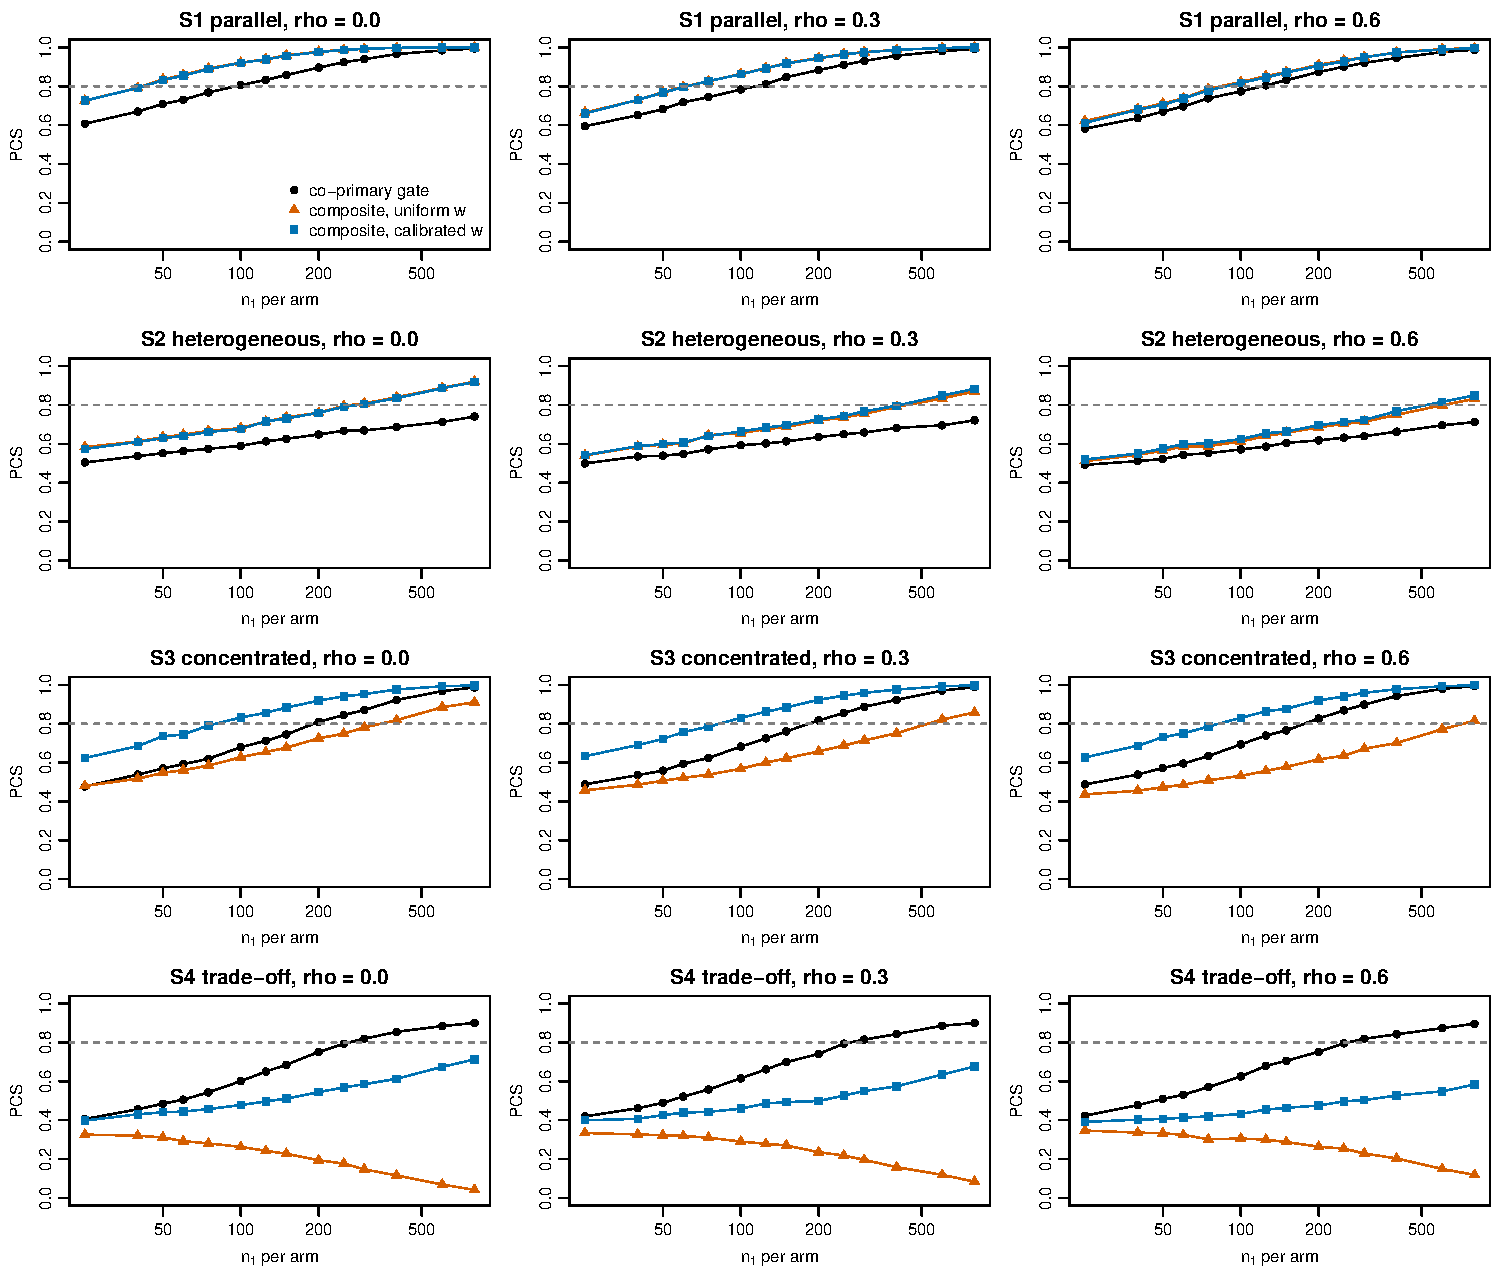
\includegraphics[width=\textwidth]{sim_fig.pdf}
\caption{Probability of correct selection against stage-1 sample size per arm, for the four configurations of Table~\ref{tab:scen} and three latent correlations. The horizontal line marks $\PCS^\ast=0.8$. In S4 the uniform-weight composite is discordant and its $\PCS$ decreases in $n_1$.}\label{fig:pcs}
\end{figure}

\begin{table}
\centering\footnotesize
\caption{Dependence on the number of doses, S1 parallel with adjacent dose effects spaced by 0.05, $\rho_{\mathrm{lat}}=0.3$, uniform weights. $\Delta N=(M-1)(n_1^{\mathrm{M}}-n_1^{\mathrm{C}})$ is the reduction in total sample size implied by \eqref{eq:accounting}.}\label{tab:msweep}
%% Generated by R/make_tables.R from results/*.csv; do not edit by hand.
\begin{tabular}{ccccc}
\toprule
$M$ & $n_1^{\mathrm{M}}$ & $n_1^{\mathrm{C}}$ & Ratio & $\Delta N$ \\
\midrule
2 & 97 (2.4) & 56 (2.1) & 0.57 & 42 \\
3 & 110 (3.0) & 63 (2.0) & 0.57 & 94 \\
4 & 102 (2.6) & 59 (1.0) & 0.57 & 131 \\
5 & 98 (1.9) & 58 (1.1) & 0.60 & 157 \\
\bottomrule
\end{tabular}

\end{table}

Table~\ref{tab:main} and Figure~\ref{fig:pcs} give the stage-1 sizes at which each gate reaches $\PCS^\ast=0.8$. Under parallel effects (S1) the composite gate needs 44--73\% of the conjunctive stage-1 size, and the observed ratio lies inside the bracket \eqref{eq:bracket} at each correlation; the saving diminishes as the endpoints become more strongly correlated, since the composite then averages less independent information. Under the heterogeneous configuration (S2) the conjunctive gate does not reach the target within 800 subjects per arm, because the two leading doses are separated by only $0.01$ on their binding endpoint, whereas the composite, which pools a separation of $0.0175$ across endpoints with lower variance, reaches it at 267--607 with uniform weights and 284--532 with configuration-specific weights. Under the concentrated configuration (S3) uniform weights dilute the signal on endpoint 1 and the composite needs 1.8 to 4.1 times the conjunctive size, while configuration-specific weights, which load 0.9--1.0 on endpoint 1, reduce it to 0.42--0.47 of the conjunctive size. Under the trade-off configuration (S4) uniform weights are discordant and $\PCS$ falls with $n_1$; configuration-specific weights restore concordance but with a margin of about $0.01$ on the composite scale, and the composite does not reach the target within the grid while the conjunctive gate does at 260--265. The ratio is stable in $M$ (Table~\ref{tab:msweep}, 0.57--0.60) and the total reduction grows with $M-1$, as \eqref{eq:accounting} implies.

\begin{table}
\centering\footnotesize
\caption{Jointly calibrated weights from \eqref{eq:weights} over a scenario set $\Theta$ ($n_1=100$, $\rho_{\mathrm{lat}}=0.3$), with the mean $\PCS$ over $\Theta$ of the resulting composite gate and of the co-primary gate on the calibration sample.}\label{tab:wjoint}
%% Generated by R/make_tables.R from results/*.csv; do not edit by hand.
\begin{tabular}{lcccccc}
\toprule
& \multicolumn{4}{c}{$\bw^\star$} & \multicolumn{2}{c}{Mean PCS over $\Theta$} \\
\cmidrule(lr){2-5}\cmidrule(lr){6-7}
Scenario set $\Theta$ (constraint) & $w_1$ & $w_2$ & $w_3$ & $w_4$ & composite $\bw^\star$ & co-primary gate \\
\midrule
$\Theta_{\mathrm{all}}=\{$S1, S2, S3, S4$\}$ & 0.50 & 0.10 & 0.00 & 0.40 & 0.651 & 0.668 \\
$\Theta_{\mathrm{conc}}=\{$S1, S2, S3$\}$ & 0.50 & 0.20 & 0.10 & 0.20 & 0.745 & 0.686 \\
$\Theta_{\mathrm{all}}$, $w_k\ge0.10$ & 0.40 & 0.10 & 0.10 & 0.40 & 0.647 & 0.668 \\
\bottomrule
\end{tabular}

\end{table}

\begin{table}
\centering\footnotesize
\caption{Cross-evaluation at $n_1=100$, $\rho_{\mathrm{lat}}=0.3$: probability of correct selection and expected regret on the co-primary scale, $100\times\E[\min_k\theta_{a^\circ,k}-\min_k\theta_{a^\star,k}]$, for the co-primary gate and for the composite gate with each weight vector, on each configuration ($20{,}000$ trials per cell on common stage-1 data; Monte Carlo standard error of a $\PCS$ at most $0.0035$). Each configuration-specific vector $\bw^\star(\mathrm{S}j)$ is evaluated off its calibration configuration as well as on it.}\label{tab:cross}
%% Generated by R/make_tables.R from results/*.csv; do not edit by hand.
\setlength{\tabcolsep}{3pt}
\begin{tabular}{llccccccc}
\toprule
& & \multicolumn{1}{c}{Co-primary} & \multicolumn{6}{c}{Composite gate, weights} \\
\cmidrule(lr){3-3}\cmidrule(lr){4-9}
Configuration & & co-primary & uniform & $\bw^\star(\Theta_{\mathrm{all}})$ & $\bw^\star(\Theta_{\mathrm{conc}})$ & $\bw^\star(\Theta_{\mathrm{all}}, w_k\ge0.1)$ & $\bw^\star$(S3) & $\bw^\star$(S4) \\
\midrule
S1 parallel & PCS & 0.789 & 0.868 & 0.826 & 0.845 & 0.844 & 0.730 & 0.844 \\
 & regret $\times100$ & 1.18 & 0.69 & 0.94 & 0.82 & 0.83 & 1.59 & 0.83 \\
S2 heterogeneous & PCS & 0.588 & 0.652 & 0.645 & 0.650 & 0.649 & 0.575 & 0.652 \\
 & regret $\times100$ & 0.60 & 0.39 & 0.44 & 0.41 & 0.42 & 0.80 & 0.39 \\
S3 concentrated & PCS & 0.680 & 0.569 & 0.716 & 0.739 & 0.671 & 0.830 & 0.503 \\
 & regret $\times100$ & 2.61 & 3.97 & 2.37 & 2.14 & 2.84 & 1.30 & 4.76 \\
S4 trade-off & PCS & 0.614 & 0.288 & 0.417 & 0.252 & 0.423 & 0.184 & 0.460 \\
 & regret $\times100$ & 2.00 & 6.70 & 4.24 & 7.17 & 4.23 & 7.95 & 2.89 \\
\midrule
Mean PCS, S1--S4 &  & 0.668 & 0.594 & 0.651 & 0.622 & 0.647 & 0.580 & 0.615 \\
Mean PCS, S1--S3 &  & 0.686 & 0.696 & 0.729 & 0.745 & 0.721 & 0.712 & 0.666 \\
\bottomrule
\end{tabular}

\end{table}

The configuration-specific weights of Table~\ref{tab:weights} assume that the designer knows the configuration, so Tables~\ref{tab:wjoint} and~\ref{tab:cross} ask what calibration achieves when they do not. Three findings matter for practice. First, the advantage of the composite gate under S1--S3 is not an artefact of the weights: on S1 and S2 every weight vector in Table~\ref{tab:cross} except $\bw^\star(\mathrm{S3})$ beats the co-primary gate on both $\PCS$ and regret, and on S3 every calibrated vector does, uniform weights being the exception. In S2 the regret of the co-primary gate is $0.60\times10^{-2}$ against $0.39$--$0.44\times10^{-2}$ for the composite, so the composite's errors are also less costly. Second, the trade-off configuration S4 is lost for every weight vector: even the configuration-specific $\bw^\star(\mathrm{S4})$ reaches $\PCS=0.46$ against $0.61$ for the co-primary gate, with twice the regret, because the composite must separate doses 2 and 3 through a margin of $0.01$ on the composite scale while the co-primary gate separates them through a margin of $0.10$ on endpoint 4. Third, calibrating jointly over a set that contains S4 produces a compromise, $\bw^\star(\Theta_{\mathrm{all}})=(0.50,0.10,0.00,0.40)$, whose mean $\PCS$ over S1--S4 ($0.651$) falls short of the co-primary gate ($0.668$) because the gain on S1--S3 ($0.73$ against $0.69$) does not pay for the loss on S4; calibrating over the concordant set gives $\bw^\star(\Theta_{\mathrm{conc}})=(0.50,0.20,0.10,0.20)$ and a mean $\PCS$ of $0.745$ against $0.686$ on S1--S3, at the price of $0.25$ on S4. Imposing the floor $w_k\ge0.1$ costs little ($0.647$ against $0.651$ over S1--S4) and avoids weights that ignore an endpoint altogether. The calibrated vectors are themselves estimates from $2{,}000$ trials per configuration and a grid of step $0.05$, and the small differences between, say, $\bw^\star(\Theta_{\mathrm{all}})$ and its floored version in Table~\ref{tab:cross} are within that resolution; what is robust is the ordering of gates within each configuration. These results turn the choice of gate into a question about the scenario set: the composite gate is the better selector when the plausible configurations are concordant, and the co-primary gate when a trade-off between endpoints is a serious possibility, a distinction that Section~\ref{sec:rule} makes operational.

\subsection{Error control}\label{sec:error}

\begin{table}
\centering\footnotesize
\caption{Run A, null configurations ($n_1=100$, $40{,}000$ trials per cell): probability of proceeding to stage 2 and probability of a false co-primary claim, by design and latent correlation. The nominal level is $\alpha=0.025$; the Monte Carlo standard error of an error rate near $0.025$ is $0.0008$.}\label{tab:e2eN}
%% Generated by R/make_tables.R from results/*.csv; do not edit by hand.
\setlength{\tabcolsep}{4pt}
\begin{tabular}{llcccccc}
\toprule
& & \multicolumn{3}{c}{$\Pr(\text{proceed})$} & \multicolumn{3}{c}{$\Pr(\text{false claim})$} \\
\cmidrule(lr){3-5}\cmidrule(lr){6-8}
Configuration & Design & $\rho_{\mathrm{lat}}=0$ & $0.3$ & $0.6$ & $\rho_{\mathrm{lat}}=0$ & $0.3$ & $0.6$ \\
\midrule
N0 global null & M: co-primary gate & 0.19 & 0.19 & 0.23 & 0.0000 & 0.0000 & 0.0003 \\
 & C: composite, uniform $\mathbf w$ & 0.17 & 0.17 & 0.22 & 0.0000 & 0.0000 & 0.0003 \\
 & C: composite, $\mathbf w^\star(\Theta_{\mathrm{all}})$ & 0.23 & 0.22 & 0.21 & 0.0000 & 0.0000 & 0.0000 \\
 & C: composite, $\mathbf w^\star$(S3) & 0.20 & 0.20 & 0.18 & 0.0000 & 0.0000 & 0.0000 \\
 & C: composite, $\mathbf w^\star$(S4) & 0.19 & 0.20 & 0.20 & 0.0000 & 0.0000 & 0.0000 \\
\addlinespace[3pt]
N1 endpoint-4 null & M: co-primary gate & 0.70 & 0.62 & 0.58 & 0.0090 & 0.0125 & 0.0123 \\
 & C: composite, uniform $\mathbf w$ & 0.98 & 0.91 & 0.86 & 0.0092 & 0.0120 & 0.0132 \\
 & C: composite, $\mathbf w^\star(\Theta_{\mathrm{all}})$ & 0.87 & 0.80 & 0.75 & 0.0115 & 0.0100 & 0.0160 \\
 & C: composite, $\mathbf w^\star$(S3) & 0.87 & 0.86 & 0.85 & 0.0090 & 0.0127 & 0.0163 \\
 & C: composite, $\mathbf w^\star$(S4) & 0.75 & 0.67 & 0.62 & 0.0105 & 0.0110 & 0.0140 \\
\addlinespace[3pt]
N2 doses 1-2 null & M: co-primary gate & 0.95 & 0.92 & 0.90 & 0.0000 & 0.0000 & 0.0000 \\
 & C: composite, uniform $\mathbf w$ & 1.00 & 0.98 & 0.94 & 0.0000 & 0.0000 & 0.0000 \\
 & C: composite, $\mathbf w^\star(\Theta_{\mathrm{all}})$ & 0.97 & 0.94 & 0.90 & 0.0000 & 0.0000 & 0.0000 \\
 & C: composite, $\mathbf w^\star$(S3) & 0.84 & 0.84 & 0.82 & 0.0000 & 0.0000 & 0.0000 \\
 & C: composite, $\mathbf w^\star$(S4) & 0.99 & 0.97 & 0.92 & 0.0000 & 0.0000 & 0.0000 \\
\addlinespace[3pt]
N3 staggered null & M: co-primary gate & 0.88 & 0.78 & 0.69 & 0.0195 & 0.0245 & 0.0235 \\
 & C: composite, uniform $\mathbf w$ & 1.00 & 0.98 & 0.94 & 0.0185 & 0.0213 & 0.0182 \\
 & C: composite, $\mathbf w^\star(\Theta_{\mathrm{all}})$ & 0.99 & 0.98 & 0.96 & 0.0105 & 0.0185 & 0.0195 \\
 & C: composite, $\mathbf w^\star$(S3) & 0.93 & 0.93 & 0.91 & 0.0115 & 0.0143 & 0.0185 \\
 & C: composite, $\mathbf w^\star$(S4) & 0.99 & 0.98 & 0.97 & 0.0120 & 0.0165 & 0.0195 \\
\addlinespace[3pt]
N4 staggered null, large effects & M: co-primary gate & 0.90 & 0.81 & 0.72 & 0.0290 & 0.0220 & 0.0227 \\
 & C: composite, uniform $\mathbf w$ & 1.00 & 1.00 & 1.00 & 0.0208 & 0.0195 & 0.0192 \\
 & C: composite, $\mathbf w^\star(\Theta_{\mathrm{all}})$ & 1.00 & 1.00 & 1.00 & 0.0107 & 0.0140 & 0.0140 \\
 & C: composite, $\mathbf w^\star$(S3) & 1.00 & 1.00 & 1.00 & 0.0125 & 0.0150 & 0.0180 \\
 & C: composite, $\mathbf w^\star$(S4) & 1.00 & 1.00 & 1.00 & 0.0125 & 0.0168 & 0.0185 \\
\bottomrule
\end{tabular}

\end{table}

\begin{table}
\centering\footnotesize
\caption{The closed test of Section~\ref{sec:final} (``union'': non-selected doses enter through $q^{(1)}_a=\max_k p^{(1)}_{a,k}$) against closing each endpoint separately (``per endpoint'': non-selected doses enter through $p^{(1)}_{a,k}$), at $n_1=100$: false-claim rate in N1 and N3, and power in S1 and S3. Nominal level $\alpha=0.025$.}\label{tab:closure}
%% Generated by R/make_tables.R from results/*.csv; do not edit by hand.
\setlength{\tabcolsep}{3.5pt}
\begin{tabular}{lllcccccc}
\toprule
& & & \multicolumn{2}{c}{$\rho_{\mathrm{lat}}=0.0$} & \multicolumn{2}{c}{$\rho_{\mathrm{lat}}=0.3$} & \multicolumn{2}{c}{$\rho_{\mathrm{lat}}=0.6$} \\
\cmidrule(lr){4-5}\cmidrule(lr){6-7}\cmidrule(lr){8-9}
Configuration & Quantity & Design & per endpoint & union & per endpoint & union & per endpoint & union \\
\midrule
N1 endpoint-4 null & false claim & M: co-primary gate & 0.0105 & 0.0083 & 0.0152 & 0.0118 & 0.0143 & 0.0165 \\
 & false claim & C: composite, uniform $\mathbf w$ & 0.0177 & 0.0123 & 0.0187 & 0.0125 & 0.0177 & 0.0127 \\
\addlinespace[3pt]
N3 staggered null & false claim & M: co-primary gate & 0.0490 & 0.0213 & 0.0473 & 0.0245 & 0.0503 & 0.0220 \\
 & false claim & C: composite, uniform $\mathbf w$ & 0.0352 & 0.0165 & 0.0398 & 0.0170 & 0.0398 & 0.0203 \\
\addlinespace[3pt]
N4 staggered null, large effects & false claim & M: co-primary gate & 0.0580 & 0.0205 & 0.0542 & 0.0227 & 0.0570 & 0.0205 \\
 & false claim & C: composite, uniform $\mathbf w$ & 0.0270 & 0.0177 & 0.0385 & 0.0195 & 0.0390 & 0.0170 \\
\addlinespace[3pt]
S1 parallel & power & M: co-primary gate & 0.708 & 0.738 & 0.752 & 0.720 & 0.752 & 0.738 \\
 & power & C: composite, uniform $\mathbf w$ & 0.806 & 0.783 & 0.797 & 0.788 & 0.777 & 0.731 \\
\addlinespace[3pt]
S3 concentrated & power & M: co-primary gate & 0.736 & 0.703 & 0.734 & 0.729 & 0.736 & 0.728 \\
 & power & C: composite, uniform $\mathbf w$ & 0.677 & 0.685 & 0.659 & 0.640 & 0.631 & 0.607 \\
\bottomrule
\end{tabular}

\end{table}

In every null configuration and for every design the false-claim rate of the proposed test is at or below $0.025$ up to Monte Carlo error (Table~\ref{tab:e2eN}), as Theorem~\ref{thm:t1e} requires; the largest of the 75 estimates is $0.026$ (N4, co-primary gate, $\rho_{\mathrm{lat}}=0$), within one standard error of $\alpha$, and the selection functional does not affect the bound. Under the global null the intersection--union claim is very conservative (at most $0.0003$), since four null endpoints must all be rejected; when the null doses are null on every endpoint (N2) a false claim essentially never occurs, because the effective dose is almost always selected. The configurations that exercise the bound are N1, a single null endpoint shared by all doses with strong effects elsewhere, where the rates are $0.007$--$0.015$, and the staggered nulls N3 and N4, where they are $0.011$--$0.026$ and the bound is attained to within Monte Carlo error by the co-primary gate ($0.021$--$0.026$). The residual conservatism in N1 comes from the Simes closure and the futility rule. In N3 and N4 the intersections over the two non-selected doses are tested with near-uniform $q^{(1)}_a$, so the closure costs little, and the co-primary gate, which ranks each dose by the statistic of its own null endpoint, selects the dose whose null endpoint looks best and hands the final analysis a stage-1 $p$-value biased towards rejection; the elementary test then sits at its bound. The composite gates rank on an average over endpoints, select the null endpoint less deliberately, and remain conservative ($0.011$--$0.020$).

Table~\ref{tab:closure} isolates the role of the intersection--union $p$-values in \eqref{eq:p1I}. Under N1 the two closures behave alike, both below $\alpha$, since the null endpoint is common to all doses and $q^{(1)}_a$ and $p^{(1)}_{a,4}$ nearly coincide. Under N3 the per-endpoint closure gives false-claim rates of $0.047$--$0.052$ with the conjunctive gate and $0.031$--$0.040$ with the composite gate, that is, about twice and 1.2--1.6 times the nominal level, for the reason given in Remark~\ref{rem:perendpoint} and Appendix~\ref{app:counter}; the conjunctive gate inflates more because its ranking statistic for each dose is essentially the statistic of that dose's null endpoint. The valid closure costs power where the non-selected doses are effective but not overwhelmingly so: in S1 and S3 the claim probability is lower by $0.01$--$0.04$ than under the per-endpoint closure. This is the price of control that holds for every configuration rather than for the configurations in which failure happens to occur on a common endpoint.

\subsection{End-to-end operating characteristics}\label{sec:e2e}

\begin{table}
\centering\footnotesize
\caption{Run A, equal stage-1 cost ($n_1=100$, $10{,}000$ trials per cell): probability of proceeding, probability of correct selection, probability of a correct claim (power), probability of a claim on the co-primary-optimal dose, and expected total sample size, by design and latent correlation. False-claim rates in these configurations were at most $0.006$ (S3, where $\theta_{1,1}=0$, and S4, where $\theta_{3,4}<0$).}\label{tab:e2eA}
%% Generated by R/make_tables.R from results/*.csv; do not edit by hand.
\setlength{\tabcolsep}{3.5pt}
\begin{tabular}{llccccccccc}
\toprule
& & \multicolumn{3}{c}{$\rho_{\mathrm{lat}}=0.0$} & \multicolumn{3}{c}{$\rho_{\mathrm{lat}}=0.3$} & \multicolumn{3}{c}{$\rho_{\mathrm{lat}}=0.6$} \\
\cmidrule(lr){3-5}\cmidrule(lr){6-8}\cmidrule(lr){9-11}
Configuration & Design & PCS & Power & $E[N]$ & PCS & Power & $E[N]$ & PCS & Power & $E[N]$ \\
\midrule
S1 parallel & M: co-primary gate & 0.80 & 0.65 & 890 & 0.79 & 0.67 & 877 & 0.77 & 0.68 & 866 \\
 & C: composite, uniform $\mathbf w$ & 0.92 & 0.72 & 900 & 0.87 & 0.72 & 895 & 0.82 & 0.72 & 878 \\
 & C: composite, $\mathbf w^\star(\Theta_{\mathrm{all}})$ & 0.86 & 0.69 & 892 & 0.83 & 0.68 & 880 & 0.79 & 0.70 & 866 \\
\addlinespace[3pt]
S2 heterogeneous & M: co-primary gate & 0.60 & 0.37 & 883 & 0.59 & 0.41 & 863 & 0.57 & 0.46 & 846 \\
 & C: composite, uniform $\mathbf w$ & 0.69 & 0.40 & 900 & 0.64 & 0.43 & 891 & 0.62 & 0.48 & 873 \\
 & C: composite, $\mathbf w^\star(\Theta_{\mathrm{all}})$ & 0.66 & 0.37 & 891 & 0.64 & 0.42 & 878 & 0.63 & 0.47 & 863 \\
\addlinespace[3pt]
S3 concentrated & M: co-primary gate & 0.68 & 0.68 & 893 & 0.69 & 0.69 & 884 & 0.69 & 0.70 & 873 \\
 & C: composite, uniform $\mathbf w$ & 0.63 & 0.65 & 900 & 0.58 & 0.62 & 899 & 0.53 & 0.60 & 893 \\
 & C: composite, $\mathbf w^\star(\Theta_{\mathrm{all}})$ & 0.75 & 0.72 & 895 & 0.72 & 0.71 & 886 & 0.69 & 0.69 & 873 \\
 & C: composite, $\mathbf w^\star$(S3) & 0.83 & 0.66 & 792 & 0.83 & 0.66 & 788 & 0.83 & 0.68 & 790 \\
\addlinespace[3pt]
S4 trade-off & M: co-primary gate & 0.60 & 0.12 & 858 & 0.61 & 0.17 & 828 & 0.64 & 0.22 & 795 \\
 & C: composite, uniform $\mathbf w$ & 0.27 & 0.07 & 899 & 0.30 & 0.10 & 891 & 0.30 & 0.12 & 871 \\
 & C: composite, $\mathbf w^\star(\Theta_{\mathrm{all}})$ & 0.43 & 0.10 & 871 & 0.42 & 0.13 & 852 & 0.41 & 0.17 & 828 \\
 & C: composite, $\mathbf w^\star$(S4) & 0.48 & 0.12 & 876 & 0.46 & 0.15 & 849 & 0.44 & 0.18 & 827 \\
\bottomrule
\end{tabular}

\end{table}

\paragraph{Equal cost (run A).}
Where the composite carries more dose-discriminating information than the binding endpoint, the advantage at the selection stage carries through to the claim (Table~\ref{tab:e2eA}). In S1 the uniform composite raises $\PCS$ from $0.77$--$0.80$ to $0.82$--$0.92$ and power from $0.72$--$0.74$ to $0.78$--$0.79$ at essentially the same $E[N]$, and the jointly calibrated $\bw^\star(\Theta_{\mathrm{all}})$ retains about half of that gain ($\PCS$ $0.79$--$0.86$, power $0.75$); in S2 the gains are smaller but in the same direction. In S3 uniform weights lose on both $\PCS$ and power, $\bw^\star(\Theta_{\mathrm{all}})$ matches or slightly exceeds the reference on both ($\PCS$ $0.69$--$0.75$ against $0.68$--$0.69$, power $0.71$--$0.74$ against $0.70$--$0.72$), and the configuration-specific $\bw^\star(\mathrm{S3})$ raises $\PCS$ to $0.83$ but gives power $0.02$--$0.03$ below the reference ($0.68$--$0.69$ against $0.70$--$0.72$) with $E[N]$ lower by about eleven per cent. The difference in $E[N]$ arises because $\bw^\star(\mathrm{S3})$ is a single-endpoint gate and proceeds in $78$\% of trials against $95$--$99$\% for the co-primary gate, whose go decision benefits from the large effects on endpoints 2--4; the same mechanism costs it power. In S4 the reference design is better on every measure, with uniform weights discordant and both calibrated vectors concordant by too small a margin ($\PCS$ $0.41$--$0.48$ against $0.60$--$0.64$). Power is low for every design in S4 ($0.08$--$0.25$) because the optimal dose has a binding effect of only $0.08$ and dose 3, which the composite favours, is null on endpoint 4, so a claim on it counts as a false claim; those rates stay below $0.003$.

\begin{table}
\centering\footnotesize
\caption{Run B, equal selection accuracy: each design at the $n_1$ giving $\PCS=0.8$ at the selection stage (Table~\ref{tab:main}).}\label{tab:e2eB}
%% Generated by R/make_tables.R from results/*.csv; do not edit by hand.
\begin{tabular}{llcccccc}
\toprule
Configuration & $\rho_{\mathrm{lat}}$ & Design & $n_1$ & $\Pr(\text{proceed})$ & PCS & Power & $E[N]$ \\
\midrule
S1 parallel & 0.0 & M: co-primary gate & 91 & 0.958 & 0.783 & 0.710 & 860 \\
 & 0.0 & C: composite, uniform $\mathbf w$ & 41 & 0.948 & 0.795 & 0.703 & 750 \\
 & 0.3 & M: co-primary gate & 110 & 0.979 & 0.808 & 0.754 & 910 \\
 & 0.3 & C: composite, uniform $\mathbf w$ & 70 & 0.960 & 0.846 & 0.779 & 818 \\
 & 0.6 & M: co-primary gate & 124 & 0.967 & 0.790 & 0.770 & 933 \\
 & 0.6 & C: composite, uniform $\mathbf w$ & 90 & 0.963 & 0.812 & 0.785 & 861 \\
\addlinespace[3pt]
S3 concentrated & 0.0 & M: co-primary gate & 197 & 0.999 & 0.805 & 0.794 & 1094 \\
 & 0.0 & C: composite, $\mathbf w^\star$(S3) & 102 & 0.843 & 0.818 & 0.720 & 826 \\
 & 0.3 & M: co-primary gate & 196 & 0.998 & 0.824 & 0.828 & 1091 \\
 & 0.3 & C: composite, $\mathbf w^\star$(S3) & 100 & 0.834 & 0.828 & 0.710 & 817 \\
 & 0.6 & M: co-primary gate & 197 & 0.992 & 0.824 & 0.820 & 1092 \\
 & 0.6 & C: composite, $\mathbf w^\star$(S3) & 87 & 0.804 & 0.790 & 0.696 & 771 \\
\bottomrule
\end{tabular}

\end{table}

\paragraph{Equal selection accuracy (run B).}
Matching $n_1$ to $\PCS=0.8$ gives, in S1, an $E[N]$ lower by $7$--$16$\% at a power within $0.025$ of the reference (Table~\ref{tab:e2eB}); the stage-1 saving is realised almost in full. In S3 the composite reaches $\PCS=0.8$ at $n_1\approx82$, but at that size the null-calibrated futility rule stops an effective drug in $28$--$29$\% of trials and the weak stage-1 component of the combination test costs further power, so $E[N]$ is lower by $32$--$34$\% but power falls from $0.80$--$0.82$ to $0.61$--$0.63$. Equal selection accuracy is therefore not the right basis for choosing $n_1$: the stage-1 size also governs the futility decision and the stage-1 contribution to the confirmatory test.

\begin{table}
\centering\footnotesize
\caption{Run C, frontier in $n_1$ at $\rho_{\mathrm{lat}}=0.3$: co-primary gate (M) against the composite gate (C; uniform weights in S1, $\bw^\star(\mathrm{S3})$ in S3).}\label{tab:e2eC}
%% Generated by R/make_tables.R from results/*.csv; do not edit by hand.
\setlength{\tabcolsep}{4pt}
\begin{tabular}{lccccccccc}
\toprule
& & \multicolumn{4}{c}{M: co-primary gate} & \multicolumn{4}{c}{C: composite gate} \\
\cmidrule(lr){3-6}\cmidrule(lr){7-10}
Configuration & $n_1$ & $\Pr(\text{proceed})$ & PCS & Power & $E[N]$ & $\Pr(\text{proceed})$ & PCS & Power & $E[N]$ \\
\midrule
S1 parallel & 40 & 0.767 & 0.660 & 0.518 & 635 & 0.811 & 0.710 & 0.578 & 663 \\
 & 60 & 0.884 & 0.715 & 0.607 & 753 & 0.907 & 0.771 & 0.654 & 766 \\
 & 80 & 0.922 & 0.750 & 0.633 & 818 & 0.949 & 0.806 & 0.683 & 833 \\
 & 100 & 0.961 & 0.787 & 0.662 & 881 & 0.976 & 0.842 & 0.706 & 888 \\
 & 120 & 0.975 & 0.817 & 0.679 & 929 & 0.988 & 0.869 & 0.710 & 935 \\
 & 150 & 0.989 & 0.848 & 0.685 & 996 & 0.997 & 0.897 & 0.718 & 999 \\
 & 200 & 0.997 & 0.881 & 0.705 & 1099 & 0.999 & 0.932 & 0.721 & 1100 \\
\addlinespace[3pt]
S3 concentrated & 40 & 0.839 & 0.534 & 0.528 & 680 & 0.830 & 0.606 & 0.565 & 675 \\
 & 60 & 0.916 & 0.588 & 0.600 & 771 & 0.928 & 0.659 & 0.655 & 778 \\
 & 80 & 0.951 & 0.630 & 0.644 & 833 & 0.965 & 0.707 & 0.703 & 841 \\
 & 100 & 0.974 & 0.685 & 0.701 & 887 & 0.982 & 0.733 & 0.727 & 891 \\
 & 120 & 0.980 & 0.714 & 0.728 & 931 & 0.992 & 0.764 & 0.745 & 936 \\
 & 150 & 0.990 & 0.760 & 0.759 & 996 & 0.997 & 0.802 & 0.777 & 999 \\
 & 200 & 0.996 & 0.813 & 0.798 & 1099 & 1.000 & 0.834 & 0.802 & 1100 \\
\bottomrule
\end{tabular}

\end{table}

\begin{figure}
\centering
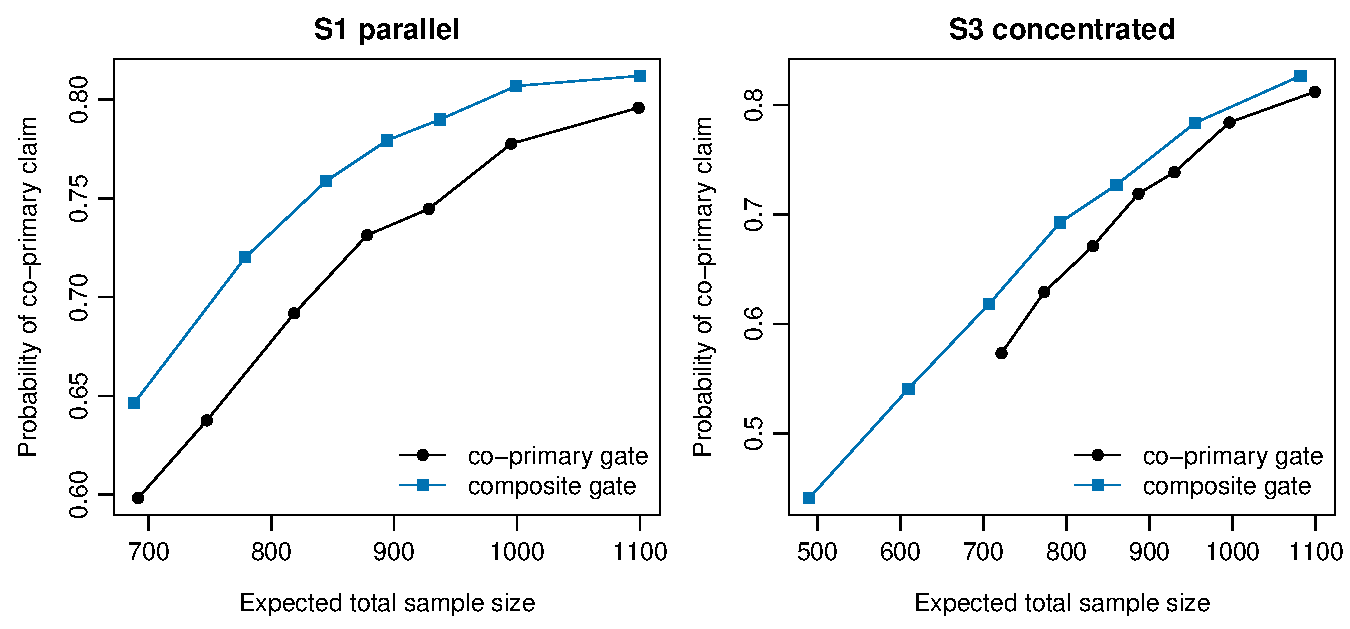
\includegraphics[width=\textwidth]{sim_e2e_fig.pdf}
\caption{Run C: probability of the co-primary claim against expected total sample size as $n_1$ varies from 40 to 200 per arm ($\rho_{\mathrm{lat}}=0.3$, $n_{\mathrm{tot}}=350$). A curve lying above and to the left dominates.}\label{fig:frontier}
\end{figure}

\begin{table}
\centering\footnotesize
\caption{Run C at matched power: stage-1 size and expected total sample size needed to reach a target claim probability, by linear interpolation of the frontiers in Table~\ref{tab:e2eC} ($\rho_{\mathrm{lat}}=0.3$). A dash marks a target not reached within $n_1\le200$.}\label{tab:e2eCm}
%% Generated by R/make_tables.R from results/*.csv; do not edit by hand.
\begin{tabular}{lcccccc}
\toprule
& & \multicolumn{2}{c}{M: co-primary gate} & \multicolumn{2}{c}{C: composite gate} & \\
\cmidrule(lr){3-4}\cmidrule(lr){5-6}
Configuration & Target power & $n_1$ & $E[N]$ & $n_1$ & $E[N]$ & $E[N]$ ratio C/M \\
\midrule
S1 parallel & 0.65 & 67 (4.9) & 772 (16.0) & 45 (3.3) & 703 (17.0) & 0.91 (0.029) \\
 & 0.70 & 90 (13.8) & 850 (47.0) & 56 (3.2) & 758 (16.0) & 0.89 (0.053) \\
 & 0.75 & 124 (14.7) & 937 (34.0) & 76 (6.8) & 834 (24.0) & 0.89 (0.041) \\
 & 0.80 & -- & -- & 120 (15.8) & 935 (35.0) & -- \\
\addlinespace[3pt]
S3 concentrated & 0.65 & 82 (4.0) & 832 (11.0) & 74 (2.7) & 716 (15.0) & 0.86 (0.021) \\
 & 0.70 & 95 (3.8) & 868 (10.0) & 90 (7.4) & 783 (27.0) & 0.90 (0.033) \\
 & 0.75 & 117 (7.2) & 924 (18.0) & 109 (3.9) & 852 (14.0) & 0.92 (0.024) \\
 & 0.80 & 185 (19.2) & 1068 (39.0) & 132 (14.6) & 925 (39.0) & 0.87 (0.048) \\
\bottomrule
\end{tabular}

\end{table}

\paragraph{Frontier (run C).}
Figure~\ref{fig:frontier} and Table~\ref{tab:e2eC} trace both designs as $n_1$ varies. Read row by row, at equal $n_1$, Table~\ref{tab:e2eC} shows the composite design with a slightly higher $E[N]$ in S1 ($894$ against $878$ at $n_1=100$). This is the futility rule: both gates proceed in $20$\% of trials under the global null, and under the alternative the composite then proceeds more often ($0.988$ against $0.956$ at $n_1=100$), so it spends the stage-2 sample more often. Since $E[N]=(M+1)n_1+2n_2\Pr(\text{proceed})$, fewer false futility stops raise $E[N]$ at fixed $n_1$; the same mechanism is part of the composite's power advantage at equal $n_1$. In S3 the sign reverses ($792$ against $887$), the single-endpoint composite proceeding less often. The comparison that matters is at equal power, and Table~\ref{tab:e2eCm} interpolates each frontier at fixed power targets. In S1 the composite reaches the same claim probability with $9$--$12$\% fewer expected subjects, the saving growing with the target because the co-primary gate's curve flattens: power $0.75$ needs $n_1=125$ and $E[N]=939$ under the co-primary gate against $n_1=75$ and $E[N]=830$ under the composite, and power $0.80$ is reached by the composite at $n_1=138$ but not by the co-primary gate within $n_1\le200$. In S3 the saving is $5$--$7$\%: the composite reaches each target at a similar $n_1$ but lower $E[N]$, because it stops more often. The S3 saving is well below the selection-stage ratio of about $0.45$: with $n_{\mathrm{tot}}$ fixed, the stage-1 saving is diluted by the confirmatory sample, and a single-endpoint composite gives a less decisive futility decision than a conjunctive gate when every endpoint responds.

\paragraph{Futility behaviour under a single null endpoint.}
Under N1 the co-primary gate proceeds in $55$--$72$\% of trials, the uniform composite in $85$--$98$\% and $\bw^\star(\Theta_{\mathrm{all}})$ in $69$--$82$\% (Table~\ref{tab:e2eN}). A composite averages a null component with three positive ones and does not register the failure; the conjunctive gate does. The final analysis protects the error rate in both cases, but the composite design spends the stage-2 sample far more often when one component is inert ($E[N]$ of $824$--$890$ against $673$--$759$ for uniform weights). This is the price of the composite gate, and it should be weighed against the selection advantage in any setting where failure on a single component is a realistic outcome.

\subsection{Design rule}\label{sec:rule}

The simulation study supports the following rule for deciding between the two gates and fixing $n_1$. For the pre-specified scenario set $\Theta$,
\begin{enumerate}[label=(\arabic*),leftmargin=*]
\item the weights $\bw^\star$ from \eqref{eq:weights} over $\Theta$, subject to the clinical constraints $\cW$ and to a floor $w_k\ge w_{\min}$ on every component so that no endpoint is ignored, must be concordant at every $\theta\in\Theta$, and the composite gate with $\bw^\star$ must have the higher $\PCS$ at every $\theta\in\Theta$ in a cross-evaluation of the kind in Table~\ref{tab:cross}; if no such $\bw$ exists, as when $\Theta$ contains a trade-off configuration, the conjunctive gate is retained;
\item the futility boundary $\eta$ is calibrated for each gate under the global null to a common probability of proceeding;
\item for each gate, $n_1$ is the smallest value at which the design attains the target claim probability at the design alternative, read from the frontier of power against $E[N]$ as in Table~\ref{tab:e2eCm}, not from selection accuracy alone, since the stage-1 size also drives the futility decision and the stage-1 weight in the combination test;
\item the composite gate is adopted only if its $E[N]$ at that point is below that of the conjunctive gate at its own smallest adequate $n_1$; where $\Theta$ gives material weight to failure on a single component, the expected sample size under that configuration enters the comparison as well.
\end{enumerate}
Whichever gate is chosen, the confirmatory analysis of Sections~\ref{sec:final} and \ref{sec:t1e} is unchanged, since the error-control argument does not depend on the gate. In the vaccine example, where a better formulation tends to be better on every serogroup and the weights can be fixed from disease burden, conditions (1) and (4) are plausible; the single-serogroup shortfall observed by {\O}stergaard et al\cite{ostergaard2009} is the configuration that condition (4) asks the design team to weigh.

\section{Discussion}\label{sec:disc}

The design studied here separates the two jobs a seamless phase II/III trial with co-primary endpoints has to do. Selection asks which dose is most likely to be the best, and a scalar weighted composite of the components, with its posterior computed exactly from the Dirichlet--multinomial model, answers that question with less data than the conjunctive criterion whenever the composite ranks the doses in the same order as the co-primary criterion. Confirmation asks whether the selected dose works on every endpoint, and that question is answered by the co-primary test with the stage-1 data included. Theorem~\ref{thm:t1e} shows that the two jobs can be given to two different functionals without any cost in type I error, provided the confirmatory closed test is built on the union hypotheses ``not effective on every endpoint'' rather than endpoint by endpoint. We regard this last point as of independent interest: a seamless design with co-primary endpoints that closes each endpoint separately, which is the natural extension of the single-endpoint methodology, does not control the false-claim rate when different candidates fail on different endpoints, and the inflation in our staggered null configuration was about twofold for the conjunctive gate. The remedy costs $0.01$--$0.04$ in power in the alternatives we studied.

The sample-size advantage of the composite is real but conditional. It is largest when dose effects are parallel and the endpoints are weakly correlated, where the bracket \eqref{eq:bracket} predicts and the simulation confirms a stage-1 saving of a half or more, and it survives the confirmatory stage as a $9$--$12$\% reduction in expected total sample size at equal power. It is smaller when the discriminating information sits on one endpoint, where calibrated weights are needed and the composite becomes a single-endpoint gate with a less decisive futility rule, and it is absent, indeed reversed, when the co-primary optimum is a trade-off between endpoints. Concordance of the weights with the co-primary criterion over the scenario set cannot be checked from the data of the trial and has to be argued from external knowledge, which in the vaccine setting is the biology of the carrier-conjugate response and the epidemiology that fixes the weights. Calibration is not a substitute for that knowledge: weights calibrated jointly over a scenario set that contained a trade-off configuration were a compromise that lost to the co-primary gate on average, while calibration over the concordant configurations gained $0.06$ in mean $\PCS$ and lost heavily on the trade-off (Table~\ref{tab:cross}). The design rule of Section~\ref{sec:rule} makes this explicit, requires a floor on every weight, which cost less than $0.005$ in mean $\PCS$ in our study, and places failure on a single component, the composite's blind spot, in the scenario set. A composite gate supplemented by a per-endpoint futility check at a lenient level would limit that blind spot at some cost in selection efficiency; the error-control argument covers any such modification.

Several limitations should be noted. The stage-wise $p$-values are Wald $p$-values, valid asymptotically; the simulated error rates show no problem at the sample sizes considered, but exact or score tests would be preferable with rare endpoints or small stage-2 samples, and Theorem~\ref{thm:t1e} accommodates them. The Simes combination requires positive regression dependence of the stage-1 statistics; this holds under the latent Gaussian dependence used here and is plausible for serogroup responses, but the Bonferroni combination should be used where negative dependence between endpoints is possible. The dependence model is a latent Gaussian threshold model with a single correlation; cell configurations with the same marginals and pairwise correlations but different higher-order structure would move the conjunction probability and the composite variance, and the Dirichlet--multinomial posterior handles them without change, but we have not studied them. The stage-2 sample size was fixed; re-estimation by predictive probability of success, \eqref{eq:ppos}, is covered by the theorem and would improve the frontier of both designs, more so for the design with the better interim information. The futility boundary was calibrated under the global null to a common probability of proceeding; other calibrations, for example to a common probability of stopping under the alternative, would shift both frontiers. Estimation for the selected dose was discussed but not evaluated; the selection bias enters the confirmatory endpoints through a different functional from the one selected on, and its size and the performance of the selection-conditional posterior \eqref{eq:selcond} are a natural subject for further work, as is the use of a hierarchical prior across doses to borrow strength at the selection stage. Finally, the simulation tested superiority; the non-inferiority margins of the motivating trial change the margins $\delta_k$ and $\gamma$ but nothing else, and a re-analysis of the formulation study of {\O}stergaard et al\cite{ostergaard2009} under the licensed margin is the intended next illustration.




\bmsection*{Acknowledgments}
Added at production.

\bmsection*{Financial disclosure}
None reported.

\bmsection*{Conflict of interest}
The author declares no potential conflict of interests.

\bmsection*{Data availability statement}
No new data were created. R code reproducing every table and figure, including the method functions, the simulation configurations and the scripts that generate the tables from the simulation output, is available at \url{https://github.com/ZerongChenNHLI/BS-CME}.

%% The class uses \doi to store the article's own DOI; give it back apacite's meaning
%% (a linked https://doi.org/ address) for the reference list.
\renewcommand{\doiprefix}{}
\renewcommand{\doi}[1]{\href{https://doi.org/#1}{https://doi.org/#1}}
\bibliography{refs}

\begin{appendix}

\section{Dirichlet aggregation and the moments of linear functionals}\label{app:dirichlet}

Let $\bpi\sim\Dir(\balpha)$ on the $J$-simplex, with $\alpha_0=\sum_j\alpha_j$, and for $\cR\subseteq\{1,\dots,J\}$ write $\pi(\cR)=\sum_{j\in\cR}\pi_j$ and $\alpha(\cR)=\sum_{j\in\cR}\alpha_j$.

\begin{lemma}[Aggregation]\label{lem:agg}
For any partition $\cR_1,\dots,\cR_L$ of $\{1,\dots,J\}$, $\big(\pi(\cR_1),\dots,\pi(\cR_L)\big)\sim\Dir\big(\alpha(\cR_1),\dots,\alpha(\cR_L)\big)$. In particular $\pi(\cR)\sim\Beta\big(\alpha(\cR),\alpha_0-\alpha(\cR)\big)$ for every $\cR$, which is \eqref{eq:beta}.
\end{lemma}

\begin{proof}
Write $\pi_j=G_j/\sum_{l}G_l$ with $G_1,\dots,G_J$ independent, $G_j\sim\mathrm{Gamma}(\alpha_j,1)$. Then $\sum_{j\in\cR_l}G_j\sim\mathrm{Gamma}(\alpha(\cR_l),1)$, the $L$ group sums are independent, and the vector of their proportions is Dirichlet with the group-sum parameters. The Beta statement is the case $L=2$.
\end{proof}

\begin{lemma}[Moments of linear functionals]\label{lem:mom}
For $\bc\in\mathbb R^J$, $\E[\bc^\top\bpi]=\bc^\top\balpha/\alpha_0$ and
\begin{equation*}
\Var[\bc^\top\bpi]=\frac{\alpha_0\sum_j c_j^2\alpha_j-\big(\sum_j c_j\alpha_j\big)^2}{\alpha_0^2(\alpha_0+1)} .
\end{equation*}
\end{lemma}

\begin{proof}
The Dirichlet moments are $\E[\pi_j]=\alpha_j/\alpha_0$ and $\Cov(\pi_j,\pi_l)=(\alpha_0\,\alpha_j\ind\{j=l\}-\alpha_j\alpha_l)/\{\alpha_0^2(\alpha_0+1)\}$, and $\Var[\bc^\top\bpi]=\sum_{j,l}c_jc_l\Cov(\pi_j,\pi_l)$.
\end{proof}

Equation \eqref{eq:moments} follows with $\bc(\bw)=\sum_k w_k\ind_{\cR_k}$ applied to the posterior $\Dir(\balpha'_a)$: $\sum_j c_j\alpha'_{a,j}=\sum_k w_k\alpha'_a(\cR_k)$, and since $\ind_{\cR_k}(j)\ind_{\cR_{k'}}(j)=\ind_{\cR_k\cap\cR_{k'}}(j)$, $\sum_j c_j^2\alpha'_{a,j}=\sum_{k,k'}w_kw_{k'}\alpha'_a(\cR_k\cap\cR_{k'})$. The same calculation with $\bc=\ind_{\cR_k}$ and $\bc=\ind_{\cR_{k'}}$ gives the posterior covariance of two component success probabilities, $\Cov(p_{a,k},p_{a,k'}\mid\bx^{(1)}_a)=\{\alpha'_{a,0}\alpha'_a(\cR_k\cap\cR_{k'})-\alpha'_a(\cR_k)\alpha'_a(\cR_{k'})\}/\{(\alpha'_{a,0})^2(\alpha'_{a,0}+1)\}$, which is the quantity the conjunctive gate and the composite gate share.

\section{Proof of Theorem~\protect\thmtone}\label{app:proof}

Throughout, $\mathcal F_1$ denotes the $\sigma$-field generated by the stage-1 data and the external information used at the interim; the selected dose $a^\star$, the go/no-go decision, $n_2$ and every $p^{(1)}_{a,k}$ are $\mathcal F_1$-measurable. A statistic $P$ with values in $[0,1]$ is called a valid $p$-value for a hypothesis $H$ if $\Pr(P\le u)\le u$ for all $u\in[0,1]$ whenever $H$ is true, and conditionally valid given $\mathcal F_1$ if $\Pr(P\le u\mid\mathcal F_1)\le u$ almost surely on the event that $H$ is true.

\begin{lemma}[Combination of valid $p$-values]\label{lem:comb}
Let $\psi_m$ be the Bonferroni combination, or the Simes combination applied to $p$-values satisfying the Simes inequality. If $P_1,\dots,P_m$ are valid $p$-values for $H_1,\dots,H_m$, then $\psi_m(P_1,\dots,P_m)$ is a valid $p$-value for $\bigcap_iH_i$. The same holds conditionally on $\mathcal F_1$: if the $P_i$ are conditionally valid and satisfy the Simes inequality conditionally, $\psi_m(P_1,\dots,P_m)$ is conditionally valid. Both combinations are non-decreasing in each argument.
\end{lemma}

\begin{proof}
For Bonferroni, $\Pr(m\min_iP_i\le u)\le\sum_i\Pr(P_i\le u/m)\le u$, and the same inequality holds for conditional probabilities. For Simes the statement is the Simes inequality\cite{simes1986}, proved by Sarkar\cite{sarkar1998} for multivariate totally positive statistics and by Benjamini and Yekutieli\cite{benjamini2001} under positive regression dependence on the subset of true hypotheses, which includes jointly normal statistics with non-negative correlations; applied to the conditional distribution given $\mathcal F_1$ it gives the conditional statement. Monotonicity is immediate from the formulas, since increasing any argument cannot decrease any order statistic.
\end{proof}

\begin{lemma}[Intersection--union $p$-value]\label{lem:iu}
If $p_1,\dots,p_K$ are valid $p$-values for $H_1,\dots,H_K$, then $q=\max_k p_k$ is a valid $p$-value for $\bigcup_k H_k$.
\end{lemma}

\begin{proof}
If $\bigcup_kH_k$ is true, some $H_{k_0}$ is true, and $\Pr(q\le u)\le\Pr(p_{k_0}\le u)\le u$.
\end{proof}

\begin{lemma}[Inverse-normal combination across stages]\label{lem:inv}
Let $P_1$ be $\mathcal F_1$-measurable and valid, and let $P_2$ be conditionally valid given $\mathcal F_1$. Then for $v_1^2+v_2^2=1$, $v_2>0$, the combination $\cC(P_1,P_2)$ of \eqref{eq:comb} satisfies $\Pr\big(\cC(P_1,P_2)\le\alpha\big)\le\alpha$.
\end{lemma}

\begin{proof}
Put $Z_i=\Phi^{-1}(1-P_i)$, so that $\cC(P_1,P_2)\le\alpha$ if and only if $v_1Z_1+v_2Z_2\ge z_{1-\alpha}$. Conditional validity gives $\Pr(Z_2\ge t\mid\mathcal F_1)=\Pr\big(P_2\le1-\Phi(t)\mid\mathcal F_1\big)\le1-\Phi(t)$ for all $t$, hence
\begin{equation*}
\Pr\big(\cC\le\alpha\big)=\E\Big[\Pr\Big(Z_2\ge\frac{z_{1-\alpha}-v_1Z_1}{v_2}\,\Big|\,\mathcal F_1\Big)\Big]\le\E\big[g(Z_1)\big],\qquad g(z)=1-\Phi\Big(\frac{z_{1-\alpha}-v_1z}{v_2}\Big),
\end{equation*}
with $g$ non-decreasing. Validity of $P_1$ gives $\Pr(Z_1\ge t)\le1-\Phi(t)$, so $Z_1$ is stochastically smaller than a standard normal variable $Z$, and $\E[g(Z_1)]\le\E[g(Z)]=\Pr(v_1Z+v_2Z'\ge z_{1-\alpha})=\alpha$ for $Z'$ standard normal and independent of $Z$.
\end{proof}

\begin{proof}[Proof of Theorem~\ref{thm:t1e}]
Fix a configuration $(\bpi_1,\dots,\bpi_M,\bpi_C)$ and let $T=\{(a,k)\in\cJ:H_{a,k}\text{ true}\}$ be the set of true elementary hypotheses. It is a fixed set, determined by the configuration alone; if it is empty there is nothing to prove. By the closure principle, the rejection of any true $H_{a,k}$, $(a,k)\in T$, requires the rejection of every intersection containing $(a,k)$, in particular of $H_T$; a false claim rejects some true $H_{a^\star,k_0}$ and is therefore such a rejection. It suffices to show that $\Pr(H_T\text{ rejected})\le\alpha$.

A trial that stops for futility rejects nothing, so the rejection event is contained in the corresponding event for the trial that always proceeds to stage 2; we work with the latter, in which stage-2 data exist on every sample path and (i) and (iii) hold as stated. By \eqref{eq:rejJ}, $H_T$ is rejected if and only if $\cC(P_1,P_2)\le\alpha$ with
\begin{equation*}
P_1:=p^{(1)}_T=\psi_{|T|}\big((p^{(1)}_{a,k})_{(a,k)\in T}\big),\qquad
P_2:=p^{(2)}_T=\psi_{|T^\star|}\big((p^{(2)}_k)_{k\in T^\star}\big),\quad T^\star=\{k:(a^\star,k)\in T\},
\end{equation*}
and $P_2=1$ when $T^\star=\emptyset$. The stage-1 component $P_1$ is $\mathcal F_1$-measurable, and it is a valid $p$-value for $H_T$ by (ii) and Lemma~\ref{lem:comb}, because every $p^{(1)}_{a,k}$ entering it tests a true hypothesis. Given $\mathcal F_1$, the selected dose $a^\star$ and hence the set $T^\star$ are fixed. On $\{T^\star\ne\emptyset\}$ every $H_{a^\star,k}$ with $k\in T^\star$ is true, so by (i) and (iii) the $p^{(2)}_k$, $k\in T^\star$, are conditionally valid given $\mathcal F_1$ and, with the conditional Simes inequality where the Simes combination is used, Lemma~\ref{lem:comb} makes $P_2$ conditionally valid. On $\{T^\star=\emptyset\}$, $P_2=1$ is trivially conditionally valid. Lemma~\ref{lem:inv} gives $\Pr(\cC(P_1,P_2)\le\alpha)\le\alpha$, which completes the proof.
\end{proof}

The argument uses the selection rule, the futility rule and $n_2$ only through their $\mathcal F_1$-measurability. What the closure over all $MK$ pairs buys is that the true intersection $H_T$ is fixed in advance: it contains each dose's own null endpoints, whichever they are, so the stage-1 component $P_1$ is a single valid $p$-value whatever dose is selected. A closure over doses on a fixed endpoint $k$ would use $\bigcap_{a}H_{a,k}$ over the doses null on $k$, a set that changes with the endpoint on which the selected dose happens to be null; Appendix~\ref{app:counter} shows what goes wrong.

\subsection{The dose-level alternative}\label{app:union}

The dose-level closure of Section~\ref{sec:final} tests the hypotheses $H^\cup_a$, $a=1,\dots,M$, by closed testing over doses, each intersection $H^\cup_I=\bigcap_{a\in I}H^\cup_a$, $I\ni a^\star$, being rejected if and only if $\cC\big(\psi_{|I|}(p^{(1)}_{a^\star,k},(q^{(1)}_a)_{a\in I\setminus\{a^\star\}}),\,p^{(2)}_k\big)\le\alpha$ for every $k$, with $q^{(1)}_a=\max_kp^{(1)}_{a,k}$.

\begin{proposition}\label{prop:union}
Under (i) and (ii) of Theorem~\ref{thm:t1e}, and the conditional validity of each $p^{(2)}_k$ in (iii), the dose-level closure satisfies $\Pr(\text{claim for }a^\star\text{ and }H^\cup_{a^\star}\text{ true})\le\alpha$ for every configuration.
\end{proposition}

\begin{proof}
Let $A_0=\{a:H^\cup_a\text{ true}\}$ and fix, for each $a\in A_0$, an endpoint $k_a$ with $H_{a,k_a}$ true. On $\{a^\star\notin A_0\}$ no claim is false. As in the proof of the theorem, pass to the trial that always proceeds. On $\{a^\star=a\}$ with $a\in A_0$, the claim requires the rejection of $H^\cup_{A_0}$, hence $\cC\big(\psi_{|A_0|}(p^{(1)}_{a,k_a},(q^{(1)}_{a'})_{a'\in A_0\setminus\{a\}}),\,p^{(2)}_{k_a}\big)\le\alpha$. Since $q^{(1)}_{a'}\ge p^{(1)}_{a',k_{a'}}$ and $\psi$ and $\cC$ are non-decreasing in each argument, this implies $\cC(P_1,P_2)\le\alpha$ with $P_1=\psi_{|A_0|}\big((p^{(1)}_{a',k_{a'}})_{a'\in A_0}\big)$, which does not depend on the selected dose, is $\mathcal F_1$-measurable and is valid for the true intersection $\bigcap_{a'\in A_0}H_{a',k_{a'}}$ by Lemma~\ref{lem:comb}, and with $P_2=p^{(2)}_{k_{a^\star}}$ on $\{a^\star\in A_0\}$ and $P_2=1$ otherwise, which is conditionally valid given $\mathcal F_1$ because $H_{a^\star,k_{a^\star}}$ is true on that event. Lemma~\ref{lem:inv} completes the proof.
\end{proof}

The dose-level closure needs no Simes inequality at stage 2 and closes over $M$ doses rather than $MK$ pairs, which is why it is more powerful than the full closure (Table~\ref{tab:closure}). Its guarantee is correspondingly weaker: it bounds the probability of a false co-primary claim, not the probability of any false rejection among the $MK$ hypotheses, so it does not protect per-endpoint statements about the selected dose that are read from the same analysis. The intersection--union $p$-values $q^{(1)}_a$ (Lemma~\ref{lem:iu}) are what make its stage-1 component valid whichever dose is selected; replacing them by the same-endpoint $p$-values $p^{(1)}_{a',k_{a^\star}}$ gives the per-endpoint closure, which is valid only if the other doses are also null on $k_{a^\star}$.

\subsection{Why the per-endpoint closure fails}\label{app:counter}

Suppose each endpoint is closed separately over doses, that is, the intersection over doses $I\ni a^\star$ on endpoint $k$ is tested by $\cC\big(\psi_{|I|}((p^{(1)}_{a,k})_{a\in I}),\,p^{(2)}_k\big)$, and consider a configuration in which every dose is null on exactly one endpoint, dose $a$ on endpoint $k_a$, with $k_a\ne k_b$ for $a\ne b$ and effects on the other endpoints large enough that the corresponding $p$-values are close to zero (configurations N3 and N4 of Section~\ref{sec:sim}, with $M=3$). Then $A_0=\{1,\dots,M\}$, every claim is false, and for the selected dose $a$ and its null endpoint $k_a$ every intersection $I\ni a$ with $|I|\ge2$ contains a dose $b\ne a$ whose $p^{(1)}_{b,k_a}$ is close to zero, so that $\psi_{|I|}$ is close to zero and the intersection is rejected on endpoint $k_a$ with probability close to one. The binding condition is the elementary one, and
\begin{equation*}
\Pr(\text{false claim})\approx\sum_{a=1}^M\Pr\big(a^\star=a,\ \cC(p^{(1)}_{a,k_a},p^{(2)}_{k_a})\le\alpha\big).
\end{equation*}
If selection were independent of the stage-1 statistics of the null endpoints, each term would equal $\Pr(a^\star=a)\,\alpha$ and the sum would be $\alpha$. Selection is not independent of them: both gates favour the dose whose statistics look best in stage 1, the composite through the average of its $K$ component contrasts, of which the null endpoint is one, and the conjunctive gate through the minimum, which under this configuration is the null endpoint itself. Under the normal approximation, the stage-1 statistic $Z^{(1)}_{a,k_a}$ and the event $\{a^\star=a\}$ are positively associated, so $\Pr(a^\star=a,\,\cdot)>\Pr(a^\star=a)\Pr(\cdot)$ for each $a$ and the sum exceeds $\alpha$. For the uniform composite with $K$ equally variable, independent components the correlation between $Z^{(1)}_{a,k_a}$ and the composite contrast of dose $a$ against the other doses is $1/\sqrt{2K}$, about $0.35$ for $K=4$, diluted by the factor $v_1$ in the combination; for the conjunctive gate the ranking statistic of dose $a$ is essentially $Z^{(1)}_{a,k_a}$ itself and the association is much stronger, which is why Table~\ref{tab:closure} shows the larger inflation for that gate. Both valid closures remove the problem. In the full closure the binding intersection is $H_T$ with $T=\{(1,k_1),(2,k_2),(3,k_3)\}$, a fixed set whose stage-1 $p$-value combines three near-uniform $p$-values and is not rejected for free; in the dose-level closure the other doses enter through $q^{(1)}_b=\max_kp^{(1)}_{b,k}\ge p^{(1)}_{b,k_b}$, which is near-uniform under N3 and N4, with the same effect.

\section{Second-moment approximation for the stage-1 sample-size ratio}\label{app:bracket}

\subsection{Consistency and concordance}

Let $\hat\theta_{a,k}=\hat p_{a,k}-\hat p_{C,k}$ denote the stage-1 posterior-mean contrasts. As $n_1\to\infty$ the posterior means converge to the true probabilities and the posterior variances are of order $1/n_1$, so the composite $z$-statistic satisfies $z_a/\sqrt{n_1}\to(\bw^\top\bm\theta_a-\gamma)/\tau_a$, with $\tau_a^2$ the limit of $n_1\Var(\Delta_a\mid\bx^{(1)})$, namely the sum over the two arms of the subject-level variance of the weighted score $T$. The composite gate therefore selects, with probability tending to one, the dose maximising $(\bw^\top\bm\theta_a-\gamma)/\tau_a$. When the $\tau_a$ are equal across doses this is $a^{\mathrm C}=\arg\max_a\bw^\top\bm\theta_a$; the $\tau_a$ differ only through the dose effects on the component variances $p_{a,k}(1-p_{a,k})$, and for every configuration, correlation and weight vector in Section~\ref{sec:sim} the two maximisers coincide (the largest relative difference between the $\tau_a$ of two doses is below two per cent). Concordance, $a^{\mathrm C}=a^\circ$, is thus necessary for $\PCS\to1$, and under discordance $\PCS\to0$.

\subsection{The bracket}

Assume parallel effects $\theta_{a,k}=\theta_a$, $\delta_k=0$, uniform weights, and the normal approximation in which, for each arm $a$, $\hat p_{a,k}=p_{a,k}+\varepsilon_{a,k}$ with $\bm\varepsilon_a$ a mean-zero normal vector with common variance $\sigma^2/n_1$ and common correlation $\phi$, independent across arms. Write $\varepsilon_{a,k}=\sigma n_1^{-1/2}\big(\sqrt\phi\,U_a+\sqrt{1-\phi}\,\xi_{a,k}\big)$ with $U_a,\xi_{a,1},\dots,\xi_{a,K}$ independent standard normal, and similarly for the control with $(U_C,\xi_{C,k})$.

For the composite, $T^{\mathrm C}_a-T^{\mathrm C}_b=K^{-1}\sum_k(\hat p_{a,k}-\hat p_{b,k})$ has mean $\theta_a-\theta_b$ and variance $2\sigma^2n_1^{-1}\{\phi+(1-\phi)/K\}$, the control cancelling exactly. For the conjunctive gate, $T^{\mathrm M}_a=\min_k(\hat p_{a,k}-\hat p_{C,k})$. Ignoring the control error, $T^{\mathrm M}_a=\theta_a+\sigma n_1^{-1/2}\big(\sqrt\phi\,U_a+\sqrt{1-\phi}\min_k\xi_{a,k}\big)$, so $\E[T^{\mathrm M}_a]=\theta_a+\sigma n_1^{-1/2}\sqrt{1-\phi}\,m_K$ with $m_K=\E[\min_k\xi_{a,k}]$ common to all doses, which cancels in $\E[T^{\mathrm M}_a-T^{\mathrm M}_b]=\theta_a-\theta_b$, and $\Var[T^{\mathrm M}_a-T^{\mathrm M}_b]=2\sigma^2n_1^{-1}\{\phi+(1-\phi)V_K\}$ with $V_K=\Var[\min_k\xi_{a,k}]$. With the control error restored, $T^{\mathrm M}_a-T^{\mathrm M}_b$ acquires the term $-(e_{k_a}-e_{k_b})$, where $k_a$ and $k_b$ are the endpoints attaining the two minima and $e_k$ is the control error on endpoint $k$; this term vanishes when $k_a=k_b$ and otherwise adds variance of order $2\sigma^2n_1^{-1}(1-\phi)$, moving the factor $\phi+(1-\phi)V_K$ towards $\phi+(1-\phi)\cdot1$, the value for a single endpoint. Under the normal approximation the probability of correct selection is a function of the ratio of the pairwise signal $\theta_a-\theta_b$ to the pairwise standard deviation, so two gates reach the same $\PCS^\ast$ when $n_1$ is proportional to their variance factors; the ratio $n_1^{\mathrm C}/n_1^{\mathrm M}$ is $\{\phi+(1-\phi)/K\}/\{\phi+(1-\phi)f\}$ with $f$ between $V_K$ and $1$, which is \eqref{eq:bracket}.

The constants are $V_K=\E[\xi_{(1)}^2]-\E[\xi_{(1)}]^2$ for the minimum $\xi_{(1)}$ of $K$ independent standard normal variables, with density $K\varphi(x)\{1-\Phi(x)\}^{K-1}$: $V_2=1-1/\pi\approx0.682$, $V_3\approx0.560$ and $V_4\approx0.492$. Since $V_K$ decreases only logarithmically in $K$, $KV_K>1$ for all $K\ge2$, so the upper end of the bracket is below one whenever $\phi<1$. In the simulation study $\phi$ is evaluated at the mean control rate and a zero dose effect; the marginals there range from $0.43$ to $0.65$ across arms and endpoints, so the equal-variance assumption holds only approximately, which is one reason the bracket is wide.

\end{appendix}


\end{document}
